% !TEX TS-program = pdflatex
% !TEX root = ../Tesis.tex
%************************************************
\chapter{Spherical Brain Mapping}\label{ch:sbm}
%************************************************
\section{Introduction}
In this section we will present a feature extraction technique called \acf{SBM}. \ac{SBM} is based on the use of spherical coordinates to extract radial features from structural \ac{MRI} images. Using the features at each coordinate, we can characterize the texture in each direction, and even project the information to a bidimensional maps, which provides a significant feature reduction and a visual aid for diagnosis. 

The most basic form is the standard \ac{SBM} \cite{Martinez-Murcia2014225,Martinez-Murcia2015}, in which all voxels crossed by a rectilinear vector in a spherical coordinate pair ($\theta,\varphi$) are selected, and then, a certain measure is extracted from that set. In this sense, statistical and morphological measures such as tissue thickness, average or entropy, among others, are computed. 

Further improvements can be made to this simple approach, for example, with the layering extension \cite{Martinez-Murcia2015}, in which the mapping vector is divided in $n$ subsets containing the same number of voxels. Therefore, instead of a single map, we can obtain $n$ maps at different distances from the centre of the brain. Another useful approach is the characterization of texture features via \acf{LBP}, computed around the mapping vector, which yielded very good results in \cite{Martinez-MurciaVRLBP}.

\begin{figure*}[htp]
	\centering
	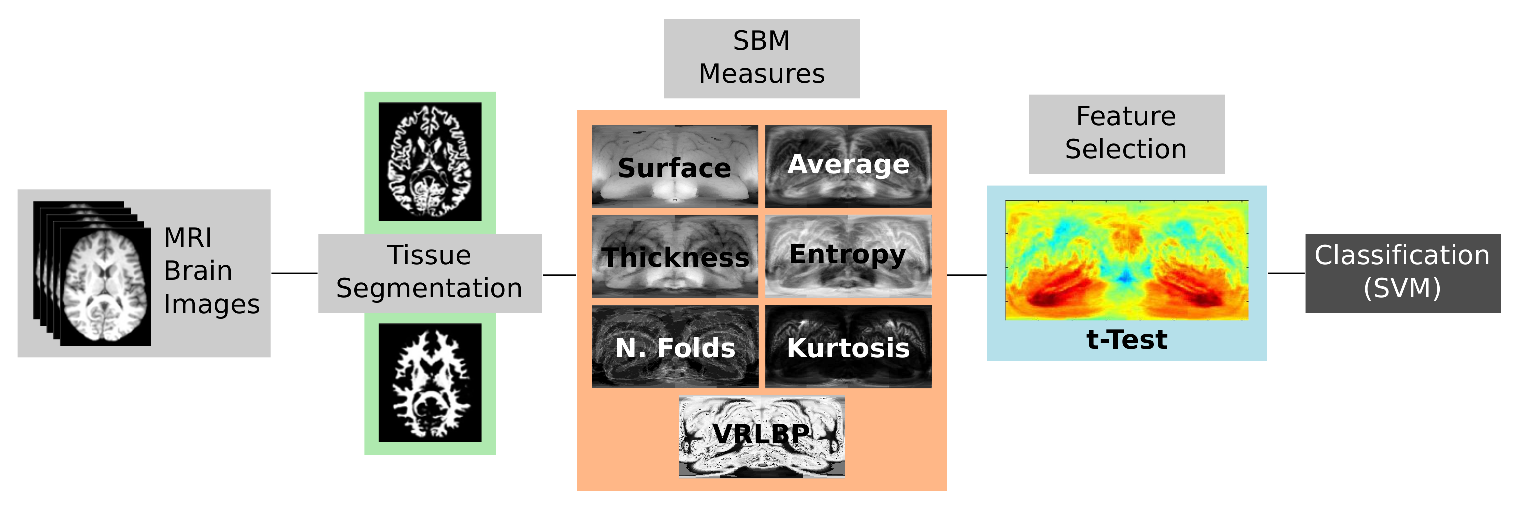
\includegraphics[width=\textwidth]{Graphics/ch6/01-flowdiagram}
	\caption{Flow diagram of the procedure used in the textural analysis of projected MR brain images.}
	\label{fig:flowdiagram}
\end{figure*}

The most relevant extension to the \ac{SBM} was proposed in \cite{Martinez-Murcia2016}. In this work, instead of using rectilinear vectors to select voxels, we developed a path creation algorithm that follows a minimum-intensity change path towards an attractor placed in its corresponding spherical coordinate pair ($\theta,\varphi$). This way, the mapping paths follow the structural features of the \ac{MRI} image, which could be used to create the bidimensional \ac{SBM} maps as well as directly use the intensity distribution along the path. This was extended to make use of the \ac{GLCM} and Haralick texture analysis (see Chapter~\ref{ch:texture}) to characterize the brain texture along each path and its neighbourhood. 


\section{\acf{SBM}}\label{sec:mapping}
The original \ac{SBM} proposed in \cite{Martinez-Murcia2014225,Martinez-Murcia2015} was based on the use of spherical coordinates in the brain. The central voxel is used as the origin point from which a number of mapping vectors $\mathbf{v}_{\theta,\varphi}$ are defined for each inclination ($\theta$) and azimuth ($\varphi$) angles in the range $0^{\circ}<\theta<180^{\circ}$ and $0^{\circ}<\varphi<360^{\circ}$ (see Figure~\ref{fig:brainmapping}). The voxels crossed by this mapping vector are selected, to form the sampled set $V_{\theta,\varphi}$, a set that contains $P$ voxels crossed by the mapping vector $\mathbf{v}_{\theta,\varphi}$.

\begin{figure}[htp]
	\centering
	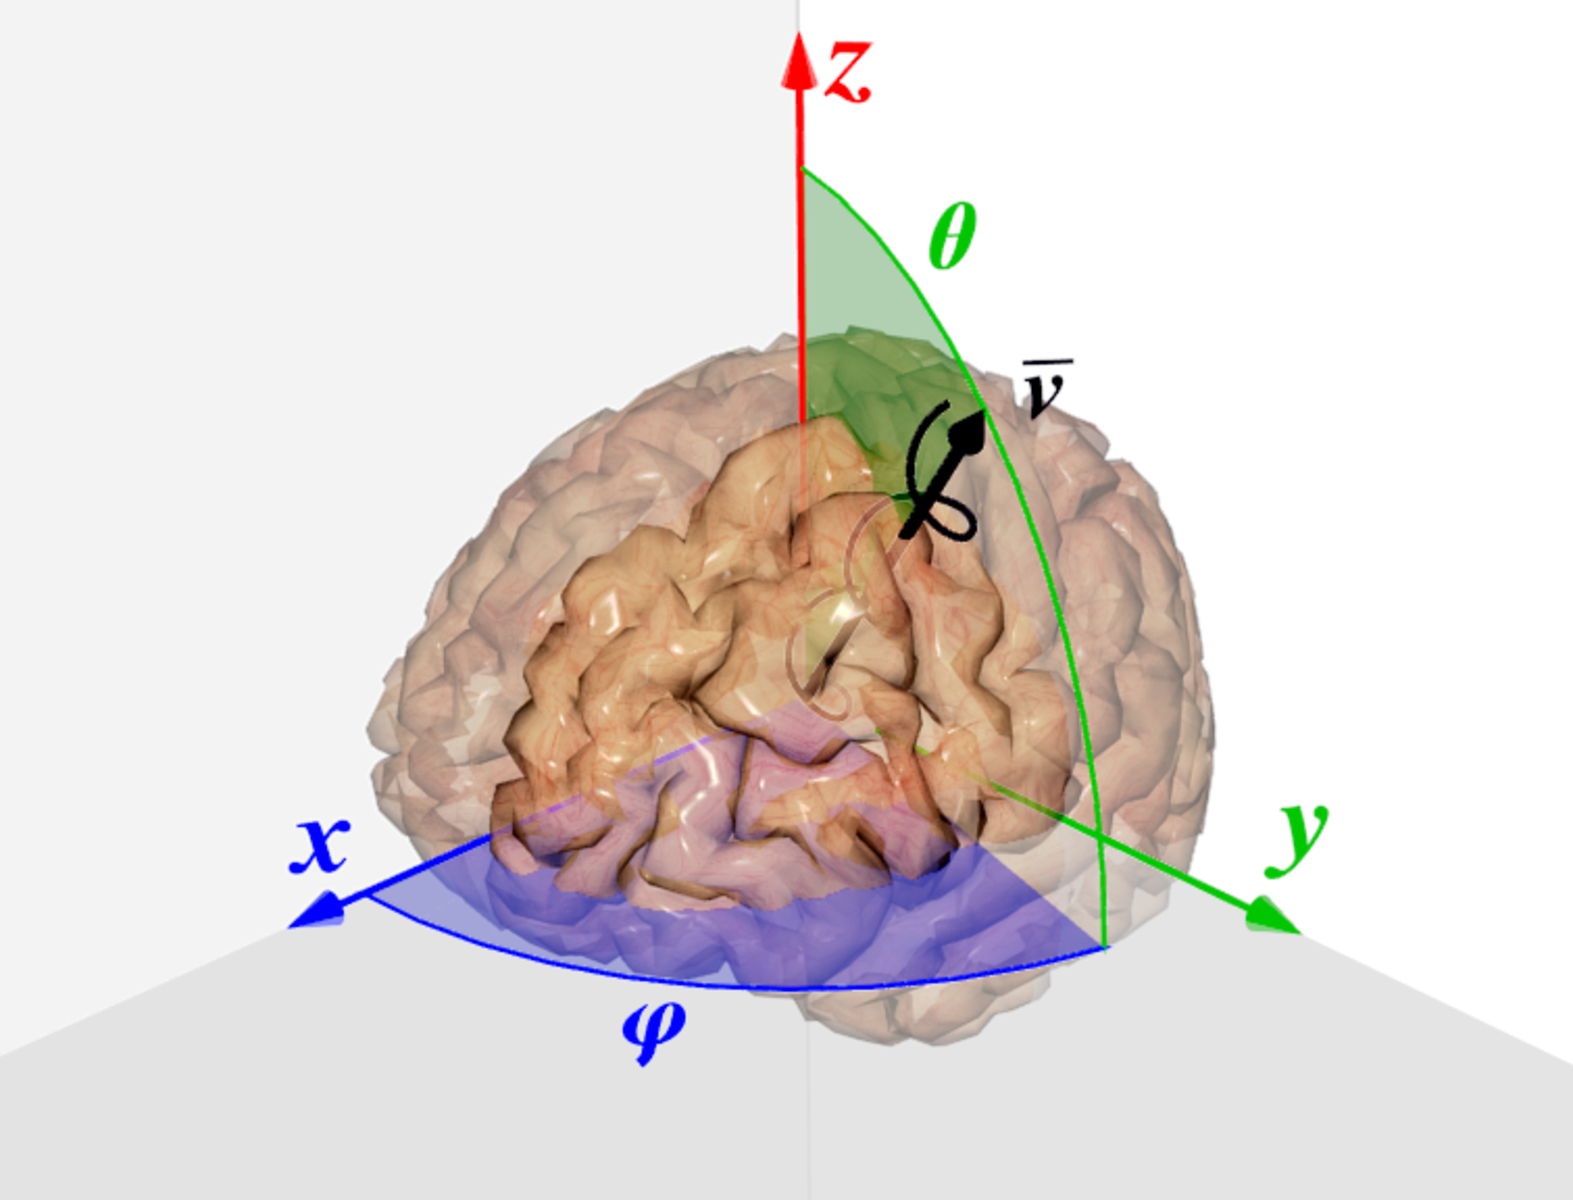
\includegraphics[width=0.7\columnwidth]{Graphics/ch6/02-projection}
	\caption{Illustration of the computation of the mapping vector $\mathbf{v}_{\theta,\varphi}$, the angles $\theta$ and $\varphi$ and the $r$-neighbourhood of $\mathbf{v}$ (see Section~\ref{sec:vrlbp}).}
	\label{fig:brainmapping}
\end{figure}

The basic form in which \ac{SBM} works is by computing a mapping value $v$ from each set $V_{\theta,\varphi}$ at each coordinate pair $(\theta,\varphi)$. In \cite{Martinez-Murcia2014225,Martinez-Murcia2015}, six basic measures were proposed: 


\begin{itemize}
	\item A basic \underline{brain surface} approach, which is intended to characterize the surface of either \ac{GM} or \ac{WM} tissue. It accounts for the distance between the origin and the last tissue voxel in $V_{\theta,\varphi}$ greater than a threshold $I_{th}$. This might correlate with structural neurodegeneration and tissue loss in the surface of the tissue. 
	\begin{equation}\label{eq:surface}
	v_{surf}= \argmax_i \lbrace V_{\theta,\varphi}(i)>I_{th}\rbrace \quad \forall i=1,\dots P
	\end{equation}  
	
	\item The \underline{thickness} of the tissue. It is defined as the distance between the last and first elements in $V_{\theta,\varphi}$
	with an intensity greater than a threshold $I_{th}$ (typically 0). This can be useful when measuring the thickness of segmented \ac{GM} or \ac{WM} maps, and, although less powerful than other implementations like Freesurfer's \cite{Dale1999}, it might be representative enough and easier to compute : 
	\begin{equation}\label{eq:thickness}
	v_{thick}=\argmax_i \lbrace V_{\theta,\varphi}(i)>I_{th}\rbrace- \argmin_i \lbrace V_{\theta,\varphi}(i)>I_{th}\rbrace
	\quad \forall i=1,\dots P
	\end{equation}  
	
	\item The \underline{number of folds} represents the number of overlapping segments of tissue in the set $V_{\theta,\varphi}$. It is computed by counting the number of connected subsets in a thresholded $V_{\theta,\varphi}$ using the value $I_{th}$. Let $A_{\theta,\varphi}$ be the set that contains all the indices of the voxels in $V_{\theta,\varphi}$ with an intensity greater than $I_{th}$:
	\begin{equation}
	A_{\theta,\varphi} = \lbrace i \; / \: V_{\theta,\varphi}(i)>I_{th} \rbrace
	\end{equation}
	where $A_{\theta,\varphi} \in \mathbb{N}$. Let us divide $A_{\theta,\varphi}$ in $J$ disjoint connected subsets so that:
	\begin{equation}
	A_{\theta,\varphi} = A_{\theta,\varphi}^1 \cup A_{\theta,\varphi}^2 \cup \dots \cup A_{\theta,\varphi}^J \quad \text{so that} \quad A_{\theta,\varphi}^i \cap A_{\theta,\varphi}^j = \emptyset \quad \forall i,j
	\end{equation}
	Therefore, our $v_{nf}=J$, the number of disjoint connected subsets in $A_{\theta,\varphi}$.
	
	\item The \underline{average} of $V_{\theta,\varphi}$: 
	\begin{equation}\label{eq:mean}
	v_{av}=\frac{1}{N}\sum_i V_{\theta,\varphi}(i) \quad \forall i=1,\dots P
	\end{equation}  
	
	\item The \underline{entropy} of $V_{\theta,\varphi}$, assuming it is a probability mass vector (probability of belonging to a certain tissue, normalized). It computes $v$ as:
	\begin{equation}
	v_{ent}=\sum_i V_{\theta,\varphi}(i)*\log(V_{\theta,\varphi}(i)) \quad \forall i \in \arg_i\lbrace V_{\theta,\varphi}(i)>0\rbrace
	\end{equation}
	
	\item The uncorrected \underline{kurtosis}, also known as fourth standardized moment, of the set $V_{\theta,\varphi}$ in which $v$ is calculated using:
	\begin{equation}
	v_{kurt}= \frac{\frac{1}{N}\sum_i\left(V_{\theta,\varphi}(i)-\bar{V}_{\theta,\varphi}(i)\right)^4}{\left(\frac{1}{N}\sum_i\left(V_{\theta,\varphi(i)}-\bar{V}_{\theta,\varphi}(i)\right)^2\right)^2} \quad \forall i=1,\dots P
	\end{equation}
	where $\bar{V}_{\theta,\varphi}$ is the average of all voxels in $V_{\theta,\varphi}$ (same value as $v_{av}$, described in Eq.~\ref{eq:mean}). 
	
\end{itemize}

We can compute each of these six maps over the \ac{GM} or \ac{WM} tissue maps of a segmented \ac{MRI}, which are depicted in Figure~\ref{fig:masksGM}. In these maps, the value $v$ computed at each direction $(\theta,\varphi)$ is represented, where the azimuth $\varphi$ is represented in the x-axis, from $0^{\circ}$ to $360^{\circ}$ and the inclination angle $\theta$ in the y-axis, from $0^{\circ}$ to $180^{\circ}$. The whole algorithm that produces these maps can be downloaded at \url{http://pakitochus.github.io/mapBrain/}.

\begin{figure*}[htp]
	\centering
	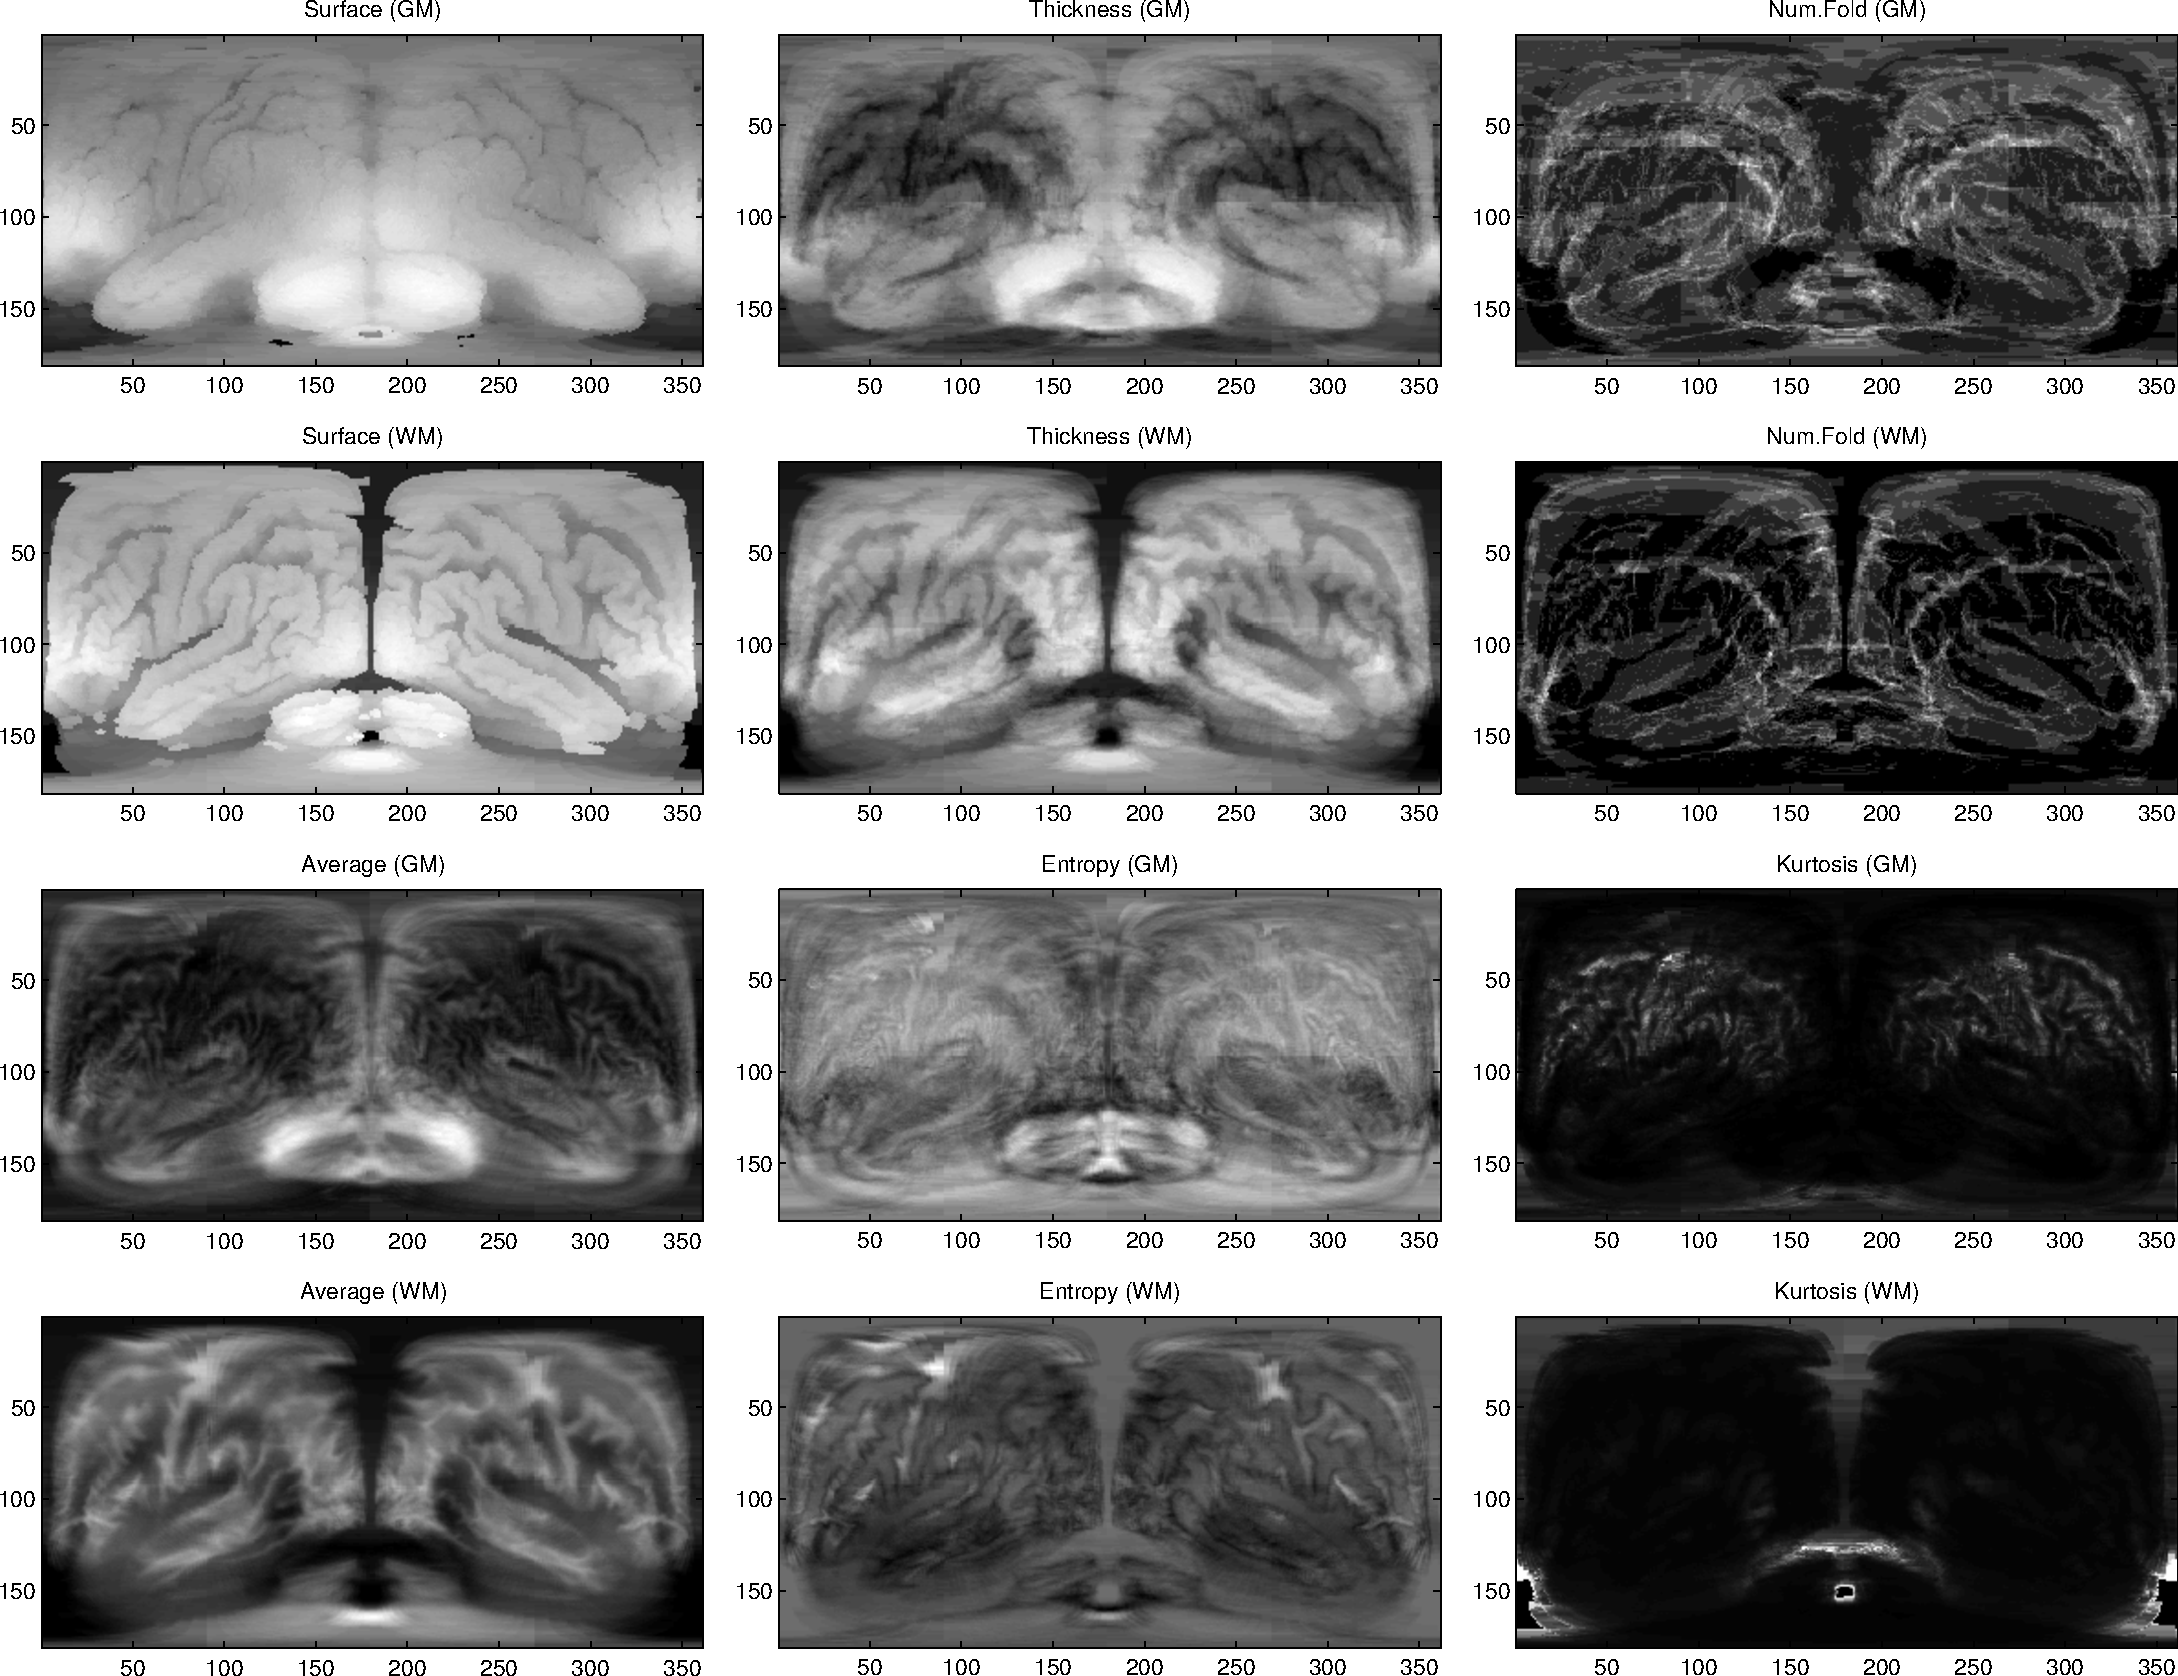
\includegraphics[width=1\textwidth]{Graphics/ch6/03-projections}
	\caption{Resulting \acs{GM} and \acs{WM} maps of the same control subject using the six proposed measures: surface, thickness, number of folds, average, entropy and kurtosis.}
	\label{fig:masksGM}
\end{figure*}

This methodology defines the sampling set as the voxels that are crossed by the sampling vector $\mathbf{v}_{\theta,\varphi}$. This implies a loss of information on the neighbourhood of $\mathbf{v}_{\theta,\varphi}$ that increases with the distance to the origin. To overcome this problem, two different approaches have been suggested. In the first one, the sampled set $V_{\theta,\varphi}$ is divided in $n$ equal parts, and one map is computed for each of the $n$ parts, in the ``Layered approach''. A second approach uses \acf{LBP} and helical sampling to map the neighbourhood of $\mathbf{v}_{\theta,\varphi}$ and characterize texture. Finally, we will define new paths that adapt to the intensity changes of the brain images, using a \ac{HMM} based approach. 

\subsection{Layered Extension}\label{sec:layered}
The layered extension is the simplest approach to keep relevant information of the different ``layers'' of tissue in our \ac{SBM} maps. To do so, we divide each sampled set $V_{\theta,\varphi}$ in $n$ equal subsets, from which $n$ maps will be derived. For example, with a $n=4$, 4 subsets will be used to compute 4 different maps at different distances from the origin, from the closest to the farthest. We assume that this approach features more detail, since overlapping structures placed at different depths will be contained within different maps. 

\begin{figure*}[htp]
	\centering
	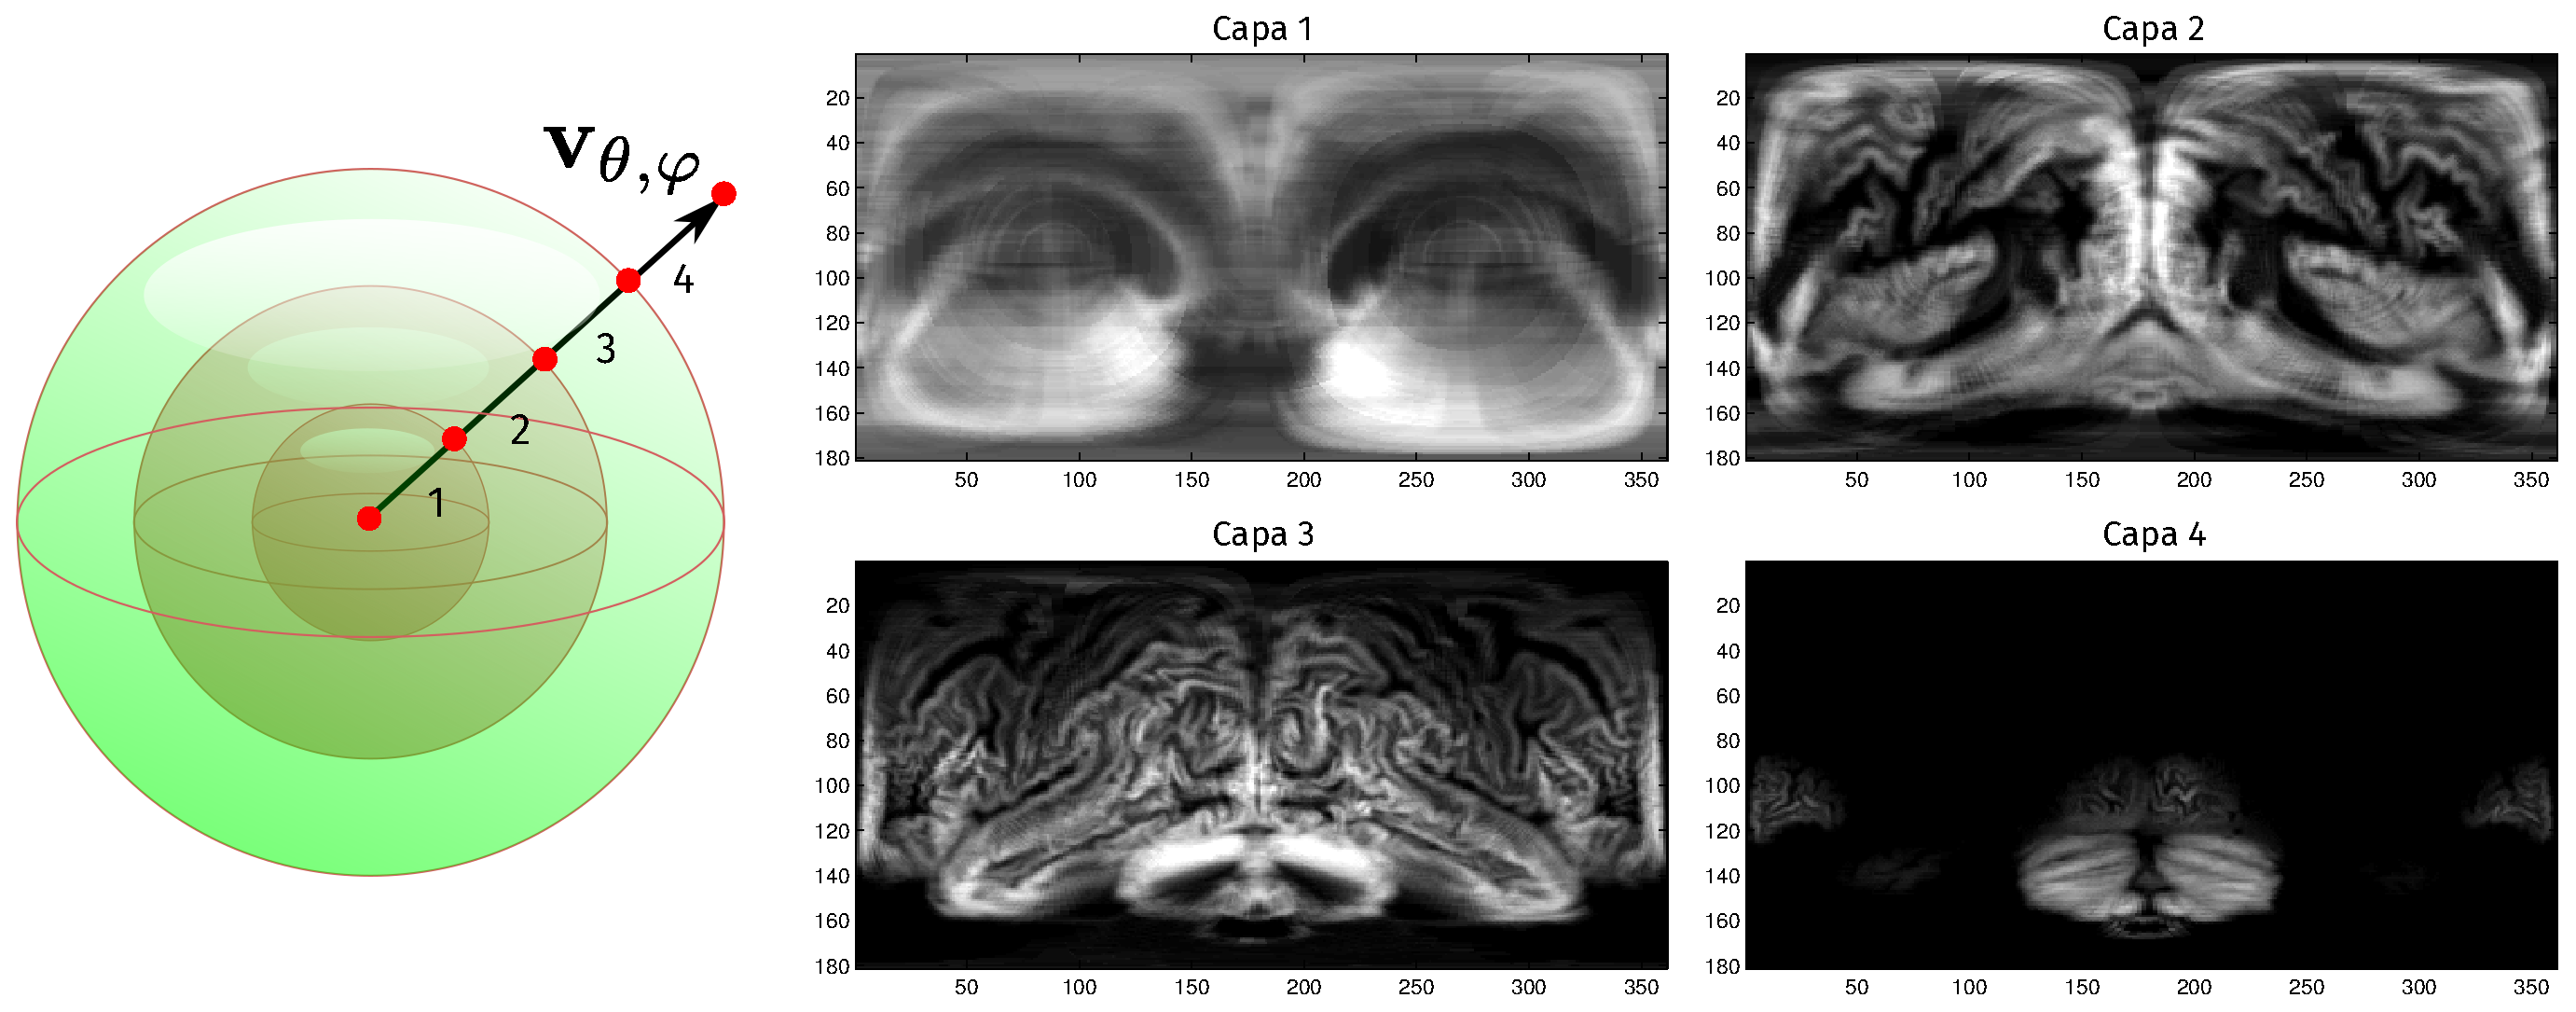
\includegraphics[width=0.9\textwidth]{Graphics/ch6/layeredAverageGM}
	\caption[Example of the layered approach using the average measure on \acs{GM} maps.]{Example of the layered approach using the average measure on \ac{GM} maps. Some internal \ac{GM} structures such as the Putamen or Globus Pallidus can be identified at Layer 2 (see anatomical reference at Figures~\ref{fig:regionsCort} and \ref{fig:regionsSub}).}
	\label{fig:layeredGM}
\end{figure*}

\subsection{\acf{VRLBP}}\label{sec:vrlbp}
Another addition that can be made to the original \ac{SBM} is the inclusion of the $r$-neighbourhood of the mapping vector $\mathbf{v}_{\theta,\varphi}$ in the computation of $v$. We do so by computing the \acf{VRLBP}, based on the \ac{LBP} descriptors proposed in \cite{Ojala1996}. 

\begin{figure*}[htp]
	\centering
	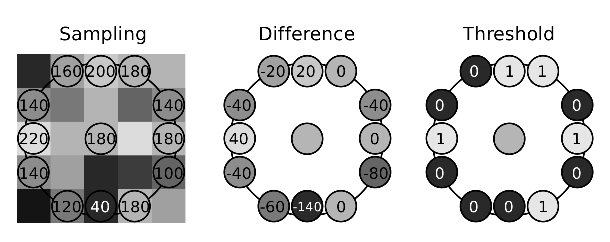
\includegraphics[width=0.8\textwidth]{Graphics/ch6/lbpLinear}
	\caption{Example of how the basic \acs{LBP} is computed.}
	\label{fig:lbpBasic}
\end{figure*}

\ac{LBP} was devised to describe the texture of a image, with an initial application to face recognition. In its basic form, it consist of three steps: sampling, calculating the difference and thresholding (See Figure~\ref{fig:lbpBasic}). The value of the \ac{LBP} is defined as:
\begin{equation}
v_{LBP} = \sum_{p=0}^{P-1} s(I_p - I_c)2^p
\end{equation}
where $P$ is the number of neighbours at a distance $r$ of the central voxel, and $I_p$ and $I_c$ are the intensities of the $p^{th}$ voxel and the central voxel for which the value $v_{LBP}$ is being computed. The threshold step is performed using the sign function $s(x)$, defined as:
\begin{equation} % He simplificado la formula usando "cases"
s(x) = 
\begin{cases}
1      &  x \geq 0 \\
0      &  x < 0
\end{cases}
\end{equation}

This basic approach was extended to Volumetric \ac{LBP} \cite{Zhao2007}, in which a 3D texture is defined in a local neighbourhood using a cylinder of radius $r$ oriented in one direction. For this work, we will update the sampling procedure proposed in \cite{Zhao2007} using a helix around the mapping vector $\mathbf{v}_{\theta,\varphi}$ (see Figure~\ref{fig:brainmapping}). This new helical sampling of \cite{Martinez-MurciaVRLBP} defines the set of $P$ sampled voxels on the image $I$ using a $r$-neighbourhood $V_{\theta,\varphi}^{P,r}$ as:

\begin{equation}
V_{\theta,\varphi}^{P,r}=\lbrace I(\mathbf{g}_{\theta,\varphi}^{0,r}), I(\mathbf{g}_{\theta,\varphi}^{1,r}), I(\mathbf{g}_{\theta,\varphi}^{2,r}), \dots I(\mathbf{g}_{\theta,\varphi}^{P-1,r})\rbrace
\end{equation} 
where the coordinate vector $\mathbf{g}_{\theta,\varphi}^{p,r}$ of each voxel are computed in the direction of $\mathbf{v}_{\theta,\varphi}$ by: 
\begin{equation}
\label{ec:helical_coordinates}
\mathbf{g}_{\theta,\varphi}^{p,r}=\begin{cases}
x_{\theta,\varphi}^{p,r}=p\sin(\varphi)\cos(\theta)-r\sin(2\pi np/P)\\
y_{\theta,\varphi}^{p,r}=p\sin(\varphi)\sin(\theta)+r\cos(2\pi np/P)\\
z_{\theta,\varphi}^{p,r}=p\cos(\varphi) 
\end{cases} \quad p=\{0,...,P-1\}, P \in \mathbb{N}
\end{equation}
being $n$ the number of turns in the helical sampling. We use linear interpolation to estimate the intensities in positions that do not fall exactly at the coordinates computed in Eq.~\ref{ec:helical_coordinates}, as in \cite{Zhao2007}. 

If we fix $P$ and $r$ to constant values, the set of sampled voxels $V_{\theta,\varphi}^{P,r}$ becomes $V_{\theta,\varphi}$, which is similar to the definition of \ac{SBM} found in Section~\ref{sec:mapping}. The value $v$ of the \ac{VRLBP} approach is therefore defined as: 
\begin{equation}
v_{VRLBP} = \sum_{p} s(V_{\theta,\varphi}(p)-V_{\theta,\varphi}(0))\cdot 2^{p} \quad \forall p=1,\dots P
\end{equation}

The resulting texture maps for \ac{GM} and \ac{WM} tissues can be found at Figure~\ref{fig:vrlbp}. 

\begin{figure*}[htp]
	\centering
	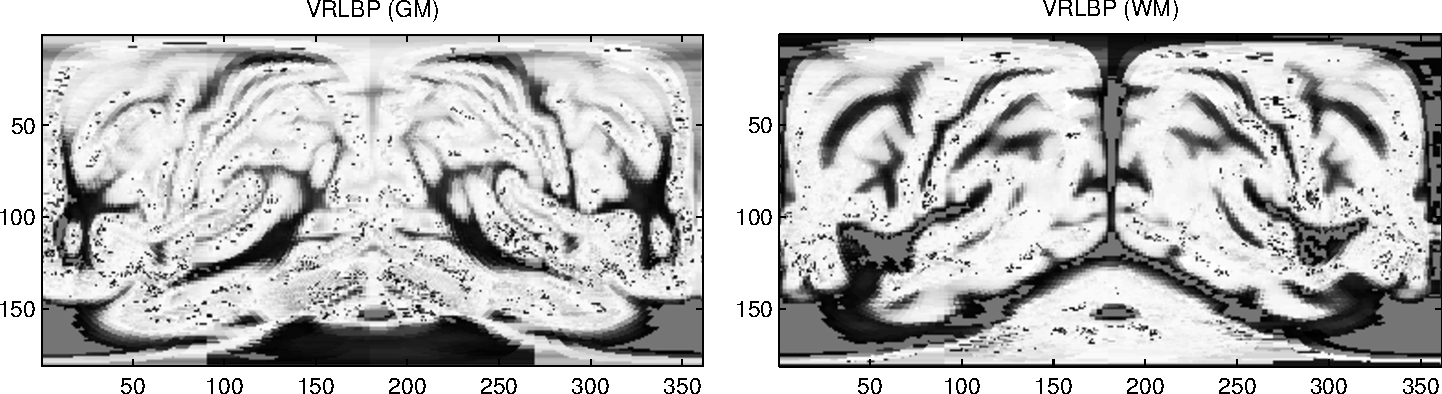
\includegraphics[width=\textwidth]{Graphics/ch6/04-vrlbp}
	\caption{An example of the \acs{VRLBP} projection for \acs{GM} and \acs{WM} Tissues. }
	\label{fig:vrlbp}
\end{figure*}

%\lstset{language=python} 
%\begin{lstlisting}
%	def foo():
%		hola amigo
%		print('amigo')
%	
%	eh = foo("amigo")
%	
%	string title = "This is a Unicode $\pi$ in the sky"
%	/*
%	Defined as $\pi=\lim_{n\to\infty}\frac{P_n}{d}$ where $P$ is the perimeter
%	of an $n$-sided regular polygon circumscribing a
%	circle of diameter $d$.
%	*/
%	const double pi = 3.1415926535
%\end{lstlisting}

\subsection{Anatomical Reference}\label{sec:anatomical}
To better understand the \ac{SBM} maps, and the location of different features, we have projected the widely known \ac{AAL} atlas \cite{Tzourio-Mazoyer2002} using \ac{SBM}. That way, we have an anatomical reference of the different structures and their position in the different coordinate pairs $(\theta,\varphi)$. The regions are displayed in  Figures~\ref{fig:regionsCort} and \ref{fig:regionsSub}. 

\begin{figure*}[htp]
	\centering
	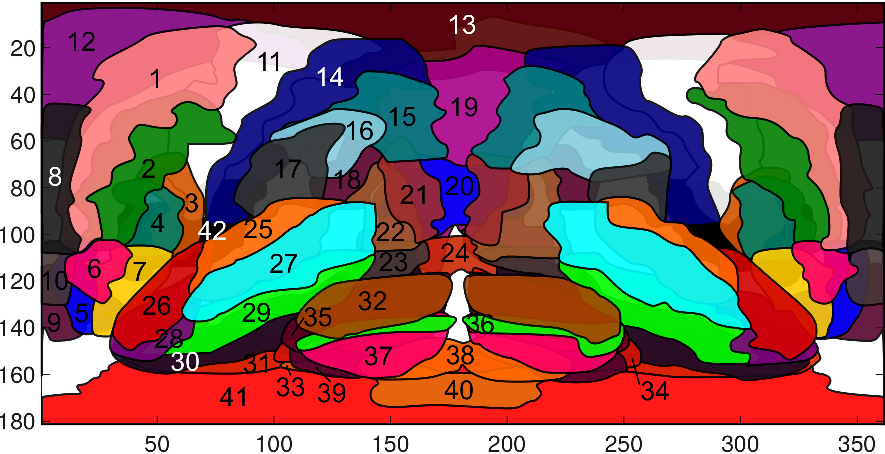
\includegraphics[width=0.7\textwidth]{Graphics/ch6/05-regions_cortical}
	
	\caption[\acs{SBM} mapping of different cortical regions.]{\ac{SBM} mapping of different cortical regions. In the Frontal region, we can find: 1) Frontal Sup., 2) Frontal Mid., 3) Frontal Inf. Oper., 4) Frontal Inf. Tri., 5) Frontal Sup. Orb, 6) Frontal Mid. Orb, 7) Frontal Inf. Orb, 8) Frontal Sup. Medial, 9) Rectus, 10) Frontal Med. Orb., 11) Precentral, 12) Supp. Motor Area. In the Parietal region: 13) Paracentral Lobe, 14) Postcentral, 15) Parietal Sup., 16) Parietal Inf., 17) Supramarginal, 18) Angular. In the Occipital region: 19) Precuneus, 20) Cuneus, 21) Occipital Sup., 22) Occipital Mid., 23) Occipital Inf., 24) Lingual. In the Temporal region: 25) Temporal Sup., 26) Temporal Pole Sup., 27) Temporal Mid., 28) Temporal Pole Mid., 29) Temporal Inf, 30) Fusiform, 31) Parahippocampal. The Cerebellum, divided in: 32) Cerebelum Crus 1, 33) Cerebelum 3, 34) Cerebelum 4-5, 35) Cerebelum 6, 36) Cerebelum 7b, 37) Cerebelum 8, 38) Cerebelum 9, 39) Cerebelum 10. And additionally, the 40) Medulla, 41) Brain Stem and 42) Insula.}
	\label{fig:regionsCort}
\end{figure*}

\begin{figure*}[htp]
	\centering
	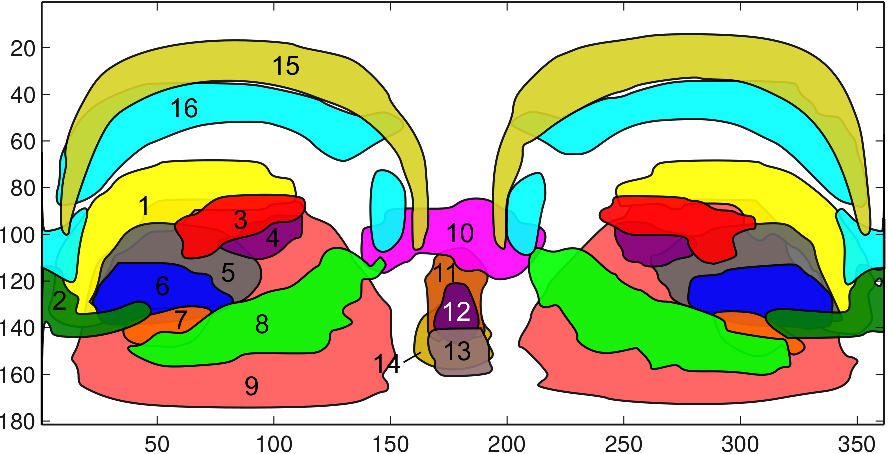
\includegraphics[width=0.7\textwidth]{Graphics/ch6/06-regions_subcortical}
	
	\caption[\acs{SBM} mapping of some subcortical regions and organs.]{\ac{SBM} mapping of of some important subcortical regions and organs. We observe the following subcortical structures: 1) Caudate Nucleus, 2) Olfactory Bulb, 3) Rolandic Operculum, 4) Heschl's gyri, 5) Putamen, 6) Globus Pallidus, 7) Amygdala, 8) Hippocampus, 9) Thalamus, 10) Lingual, 11) Vermis 4-5, 12) Vermis 7, 13) Vermis 9, 14) Vermis 1-2, 15) Cingulate Gyrus, 16) Corpus Callosum}
	\label{fig:regionsSub}
\end{figure*}

\origsection{Sampling Paths via \acfp{HMM}}\label{sec:hmmpaths}
The rectilinear mapping vector used in the original \ac{SBM} \cite{Martinez-Murcia2014225,Martinez-MurciaVRLBP,Martinez-Murcia2015} has some limitations, partially overcome by the \ac{VRLBP} and the layered extension. However, a more flexible sampling could be beneficial for the computation of texture measures. In this section we present the technique used to define minimum intensity change sampling paths via Hidden Markov Models, that was firstly proposed in \cite{Martinez-Murcia2016}. These paths are defined so that the resulting sampled sets contain information about both intensity and structure of the brain. 

% Algoritmo base de extracción de puntos
To define the paths, we consider each three-dimensional image as a tuple that contains spatial information in the image range (the coordinates $\mathbf{p} \in \mathbb{I}$) where $\mathbb{I}\subset \mathbb{R}^3$) as well as intensity information ($I(\mathbf{p}) \in \mathbb{R}$). The intensity information will be interpreted as a sampling of the underlying tissue density, and therefore, an estimation of the probability of finding tissue in each position. 

Following the notation of the \ac{VBM} defined in Section~\ref{sec:mapping}, we formulate a 3D path tracing algorithm that defines a curvilinear mapping set of positions $\mathbb{P}_{\theta,\varphi}$ directly linked to each direction $(\theta,\varphi)$ that is, at the same time, representative of the underlying intensity distribution. We then use both spatial and intensity information to construct the minimum intensity change paths oriented in the direction $(\theta,\varphi)$. Thus, we could note our 3D path in a certain direction as a Markov Model \cite{Chen2008}: 
\begin{equation}
\mathbb{P}_{\theta,\varphi} = \{\mathbf{p}_0, \mathbf{p}_1, \mathbf{p}_2, \dots \mathbf{p}_N\}
\end{equation}
Therefore, our optimum path would be the one that maximizes the probability of the path:
\begin{equation}\label{eq:optimalPath}
\mathbb{P}_{\theta,\varphi}^{opt} = \argmax_{\mathbb{P}_{\theta,\varphi}} \{P(\mathbb{P}_{\theta,\varphi})\}
\end{equation}
or its equivalent, the probability of all the nodes:
\begin{equation}\label{eq:probPath}
P(\mathbb{P}_{\theta,\varphi}) = P(\mathbf{p}_0, \mathbf{p}_1, \mathbf{p}_2, \dots \mathbf{p}_N)
\end{equation}
with $\mathbf{p}_0$ being the origin of the spherical coordinates, and $\mathbf{p}_N$ is the last possible coordinate within $\mathbb{I}$ in the current direction $(\theta,\varphi)$. In this work, we have placed $\mathbf{p}_0$ at the \ac{AC} of the image, although other options, such as setting the origin at the middle point of $\mathbb{I}$ could be considered. This choice is a convention when using the \ac{MNI} coordinates \cite{Evans1993}, sharing conectivity with both hemispheres, therefore allowing the optimal computation of our paths. If we assume a first-order \acf{HMM} for the tracing of the path, the probability of the $i$-th node in the path can be approximated as:
\begin{equation}
P(\mathbf{p}_i | \mathbf{p}_{i-1}, \mathbf{p}_{i-2}, \dots \mathbf{p}_0) \approx P(\mathbf{p}_i|\mathbf{p}_{i-1})
\end{equation}

Using this assumption, Eq.~\ref{eq:probPath} becomes:
\begin{equation}
P(\mathbb{P}_{\theta,\varphi}) = P(\mathbf{p}_0, \mathbf{p}_1, \dots \mathbf{p}_N) = \prod_{i=1}^{N} P(\mathbf{p}_i|\mathbf{p}_{i-1})
\end{equation} 

Using this \ac{HMM} definition, the hidden state of each node will be its intensity $I(\mathbf{p}_i)$. Similarly to the original \ac{SBM}, let $V_{\theta,\varphi} = \{I(\mathbf{p}_0), I(\mathbf{p}_1), \dots I(\mathbf{p}_N)\}$ be the set containing all the intensities at each node of the path. Thank to this, our optimal path (Eq.~\ref{eq:optimalPath}) can be defined as:
\begin{align}
\mathbb{P}_{\theta,\varphi}^{opt} & = \argmax_{\mathbb{P}_{\theta,\varphi}} \{P(\mathbb{P}_{\theta,\varphi}|\mathbf{I})\}\\
P(\mathbb{P}_{\theta,\varphi}|\mathbf{I}) & = P(\mathbf{p}_0, \dots x_N| I(\mathbf{p}_0), \dots I(\mathbf{p}_N))\\
& = \frac{P(I(\mathbf{p}_0), \dots I(\mathbf{p}_N)|\mathbf{p}_0, \dots \mathbf{p}_N)\cdot P(\mathbf{p}_0, \dots \mathbf{p}_N)}{P(I(\mathbf{p}_0), \dots I(\mathbf{p}_N))}\label{eq:final}
\end{align}
where:
\begin{equation}\label{eq:intP}
P(I(\mathbf{p}_0), \dots I(\mathbf{p}_N)|\mathbf{p}_0, \dots \mathbf{p}_N)  = \prod_{i=1}^{N} P (I(\mathbf{p}_i)|\mathbf{p}_i)
\end{equation}
and $P(I(\mathbf{p}_0), \dots I(\mathbf{p}_N))$ is the \textit{a priori} probability of the intensities in the path. We can ignore this term in the optimization process under the assumption that it is constant along the path, which is generally true. 

To avoid computational overload, we will define a restricted set of candidates from which we will derive all the needed probabilities. This set of candidates are defined inside the $L2$-norm support ball $B_{2,r}(\mathbf{p}-\mathbf{p}_{i-1})$ of radius $r$ centred in $\mathbf{p}_{i-1}$, resulting in the candidate set $\mathbb{P}_{\theta,\varphi}^c = \{\mathbf{p}_{c,1}, \mathbf{p}_{c,2}, \dots \mathbf{p}_{c,M} \}$. 

Individual probabilities $P (I(\mathbf{p}_i)|\mathbf{p}_i)$ needed in the computation of Eq.~\ref{eq:intP} can be computed under the assumption of a normally distributed intensity candidate set $V_{\theta,\varphi}^c$ (containing the intensities of the candidate set $\mathbb{P}_{\theta,\varphi}^c$) with mean $I(\mathbf{p}_{i-1})$ and variance $\sigma_c^2$. We will estimate the probability of the i$^{th}$ candidate node $\mathbf{p}_i$ as: 
\begin{equation}\label{eq:intensity}
P(I(\mathbf{p}_i)|\mathbf{p}_i) =\frac{1}{\sqrt{2\pi \sigma_c^2}}\exp\left(-\frac{(I(\mathbf{p}_i)-I(\mathbf{p}_{i-1}))^2}{2\sigma_c^2}\right)
\end{equation}

This support the assumption of minimal intensity change paths, since the $I(\mathbf{p}_i)$ maximizes its probability when similar to $I(\mathbf{p}_{i-1})$. 

Finally, we must restrict the direction of the computed path $\mathbb{P}_{\theta,\varphi}$, to match the definition of the \ac{SBM} framework. We do this by defining the last term $P(\mathbf{p}_0, \dots \mathbf{p}_N)$ in Eq.~\ref{eq:final}, setting an attractor located in the position $\mathbf{p}_N$, the last possible coordinate within $\mathbb{I}$ in the current direction $(\theta,\varphi)$. It should affect the transition probability between states by means of an isotropic \acf{RBF}, defined in Eq.~\ref{eq:rbf}:
\begin{align}\label{eq:rbf}
&P(\mathbf{p}_0, \dots \mathbf{p}_N) = P(\mathbf{p}_i|\mathbf{p}_N)  \\&= \frac{1}{\sqrt{(2\pi)^d|\Sigma|}} \exp\left(-\frac{1}{2}(\mathbf{p}_i-\mathbf{p}_N)\Sigma^{-1}(\mathbf{p}_i-\mathbf{p}_N)\right) 
\end{align}
where $\Sigma$ is the covariance matrix of the \ac{RBF}. For simplicity we will employ an isotropic gaussian kernel, so that $\Sigma$ is a matrix whose diagonal elements constant and equal to the euclidean distance between $\mathbf{p}_i$ and $\mathbf{p}_N$. This way, the attractor conditions the direction of the path, very slightly in the first nodes, and more strongly as it approaches the cortex, leading to a better representation of the underlying structure.  

\subsubsection{Step Size}
This algorithms considers all candidate points $\mathbf{p} \in B_{2,r}(\mathbf{p}-\mathbf{p}_i)$ for each member of the final path $\mathbb{P}_{\theta,\varphi}$. Therefore, instead of a fixed step size, we will define the radius $r$ of the support ball. To avoid computational overload while maintaining good results, we will set $r=3$, which yields approximately $200$ candidate points per iteration. 

\subsubsection{Stop Condition}
The image $\mathbb{I}$ not only contains information about the structure of the brain, but also many empty space. If the attractor is located at the last point $ \mathbf{p} \in \mathbb{I}$, we expect the resulting path to reach that point. However, what we are really interested on is the brain itself, so we define a stop condition that considers that the path is finished once it reaches the last voxel inside the brain. To do so, we use an intensity threshold. 

This threshold is calculated under the entropic thresholding, as in \cite{Yen1995}. If we note $G_m \equiv \{I_0, I_1, ... I_m\} $ the set containing all intensity levels in the image $\mathbf{I}$ (a vectorized image of length $m$), we can compute a histogram that characterizes the observed frequencies. From these frequencies we can derive the observed probability of the different grey levels. The entropic thresholding defines two distributions after normalization: 
\begin{align}
& A \equiv \left\{\frac{p_0}{P(I_{s})}, \frac{p_1}{P(I_{s})}, \dots, \frac{p_{s-1}}{P(I_{s})} \right\}\\
& B \equiv \left\{\frac{p_{s}}{1-P(I_{s})}, \frac{p_{s+1}}{1-P(I_{s})}, \dots, \frac{p_m}{1-P(I_{s})} \right\}
\end{align}
where $P(I_s) = \sum_{i}^{s}p_{I_i}$ is the cumulative density function for the $s$-th grey level. The algorithm is called entropic thresholding because we choose the threshold $I_{th}=I_s$ so that the total amount of information provided by $A$ and $B$ (which we can consider the foreground and background of the image) is maximized. Therefore, we can define the total information provided by choosing the $s$-th grey level as: 
\begin{align}
TE(s) & = E_A(s) + E_B(s) \\
& = -\sum_{i=0}^{s-1}\left(\frac{p_i}{P(I_s)}\right)\log\left(\frac{p_i}{P(I_s)}\right) \\
& - \sum_{i=s}^{m-1}\left(\frac{p_i}{1-P(I_s)}\right)\log\left(\frac{p_i}{1-P(I_s)}\right)
\end{align}

The $s$ that maximizes that latter equation is the grey level that we choose as threshold. 

A summary of our \ac{HMM}-based path tracing method is shown in Algorithm~\ref{alg:hmmPath}. In Figure~\ref{fig:cuts} we show all paths computed in all directions $(\theta,\varphi)$ for $0^o<\varphi<360^o$ and $0^o<\theta<180^o$ at an interval of $1^o$. 

\begin{algorithm*}
	\SetKwData{CandInt}{candInt}
	\SetKwData{PathList}{pathList}
	\SetKwInOut{Input}{input}
	\SetKwInOut{Output}{output}
	\Input{MRI Brain Image $I$ of size $U\times V\times W$, $\mathbf{p}_0$}
	\Output{List of nodes in the optimum path $\mathbb{P}_{\theta,\varphi}^{opt}$}
	\BlankLine
	Compute the $I_{th} = I_s$ where $s$ maximizes $TE(s)$\;
	Set $\mathbf{p}_0$ to the AC\;
	%\For{$\varphi\leftarrow -180$ \KwTo $180$}{
	%	\For{$\theta\leftarrow -90$ \KwTo $90$}{
	Compute the attractor position $\mathbf{p}_N$ in the direction $(\varphi, \theta)$\;
	$\mathbf{p}_i \leftarrow \mathbf{p}_0$\;
	\While{$(i<\text{IterLimit})$ \& $(I(\mathbf{p}_i)>I_{th})$ \& ($\mathbf{p}_i \in \mathbb{I}$)}{
		Get the node candidates $\mathbb{P}_{\theta,\varphi}^c = \{\mathbf{p}_{c,1}, \mathbf{p}_{c,2}, \dots \mathbf{p}_{c,M}\}$ where $\mathbf{p}_{c,m} \in B_{2,r}(\mathbf{p}_{c,m}-\mathbf{p}_i)$\;
		Get the intensities of the candidates $I(\mathbf{p}_c) \quad \forall \mathbf{p}_c \in \mathbb{P}_{\theta,\varphi}^c$\;
		\textbf{foreach} $\mathbf{p}_c \in \mathbb{P}_{\theta,\varphi}^c${
			compute $P(\mathbf{p}_c|\mathbf{p}_N)$ and $P(I(\mathbf{p}_c)|\mathbf{p}_i)$  \;
		}
		$\mathbf{p}_{i+1} = \argmax_{\mathbf{p}_c} [P(I(\mathbf{p}_c)|\mathbf{p}_i)\cdot P(\mathbf{p}_c|\mathbf{p}_N)]$\;
		$i=i+1$\;
	}
	$\mathbb{P}_{\theta,\varphi}^{opt}\leftarrow \{\mathbf{p}_0, \mathbf{p}_1, \dots \mathbf{p}_N\}$\; 
	%	}
	%}
	
	\caption[\acs{HMM}-based Path Creation]{\ac{HMM}-based Path Creation}\label{alg:hmmPath}
\end{algorithm*}\DecMargin{1em}


\begin{figure}
	\begin{center}
		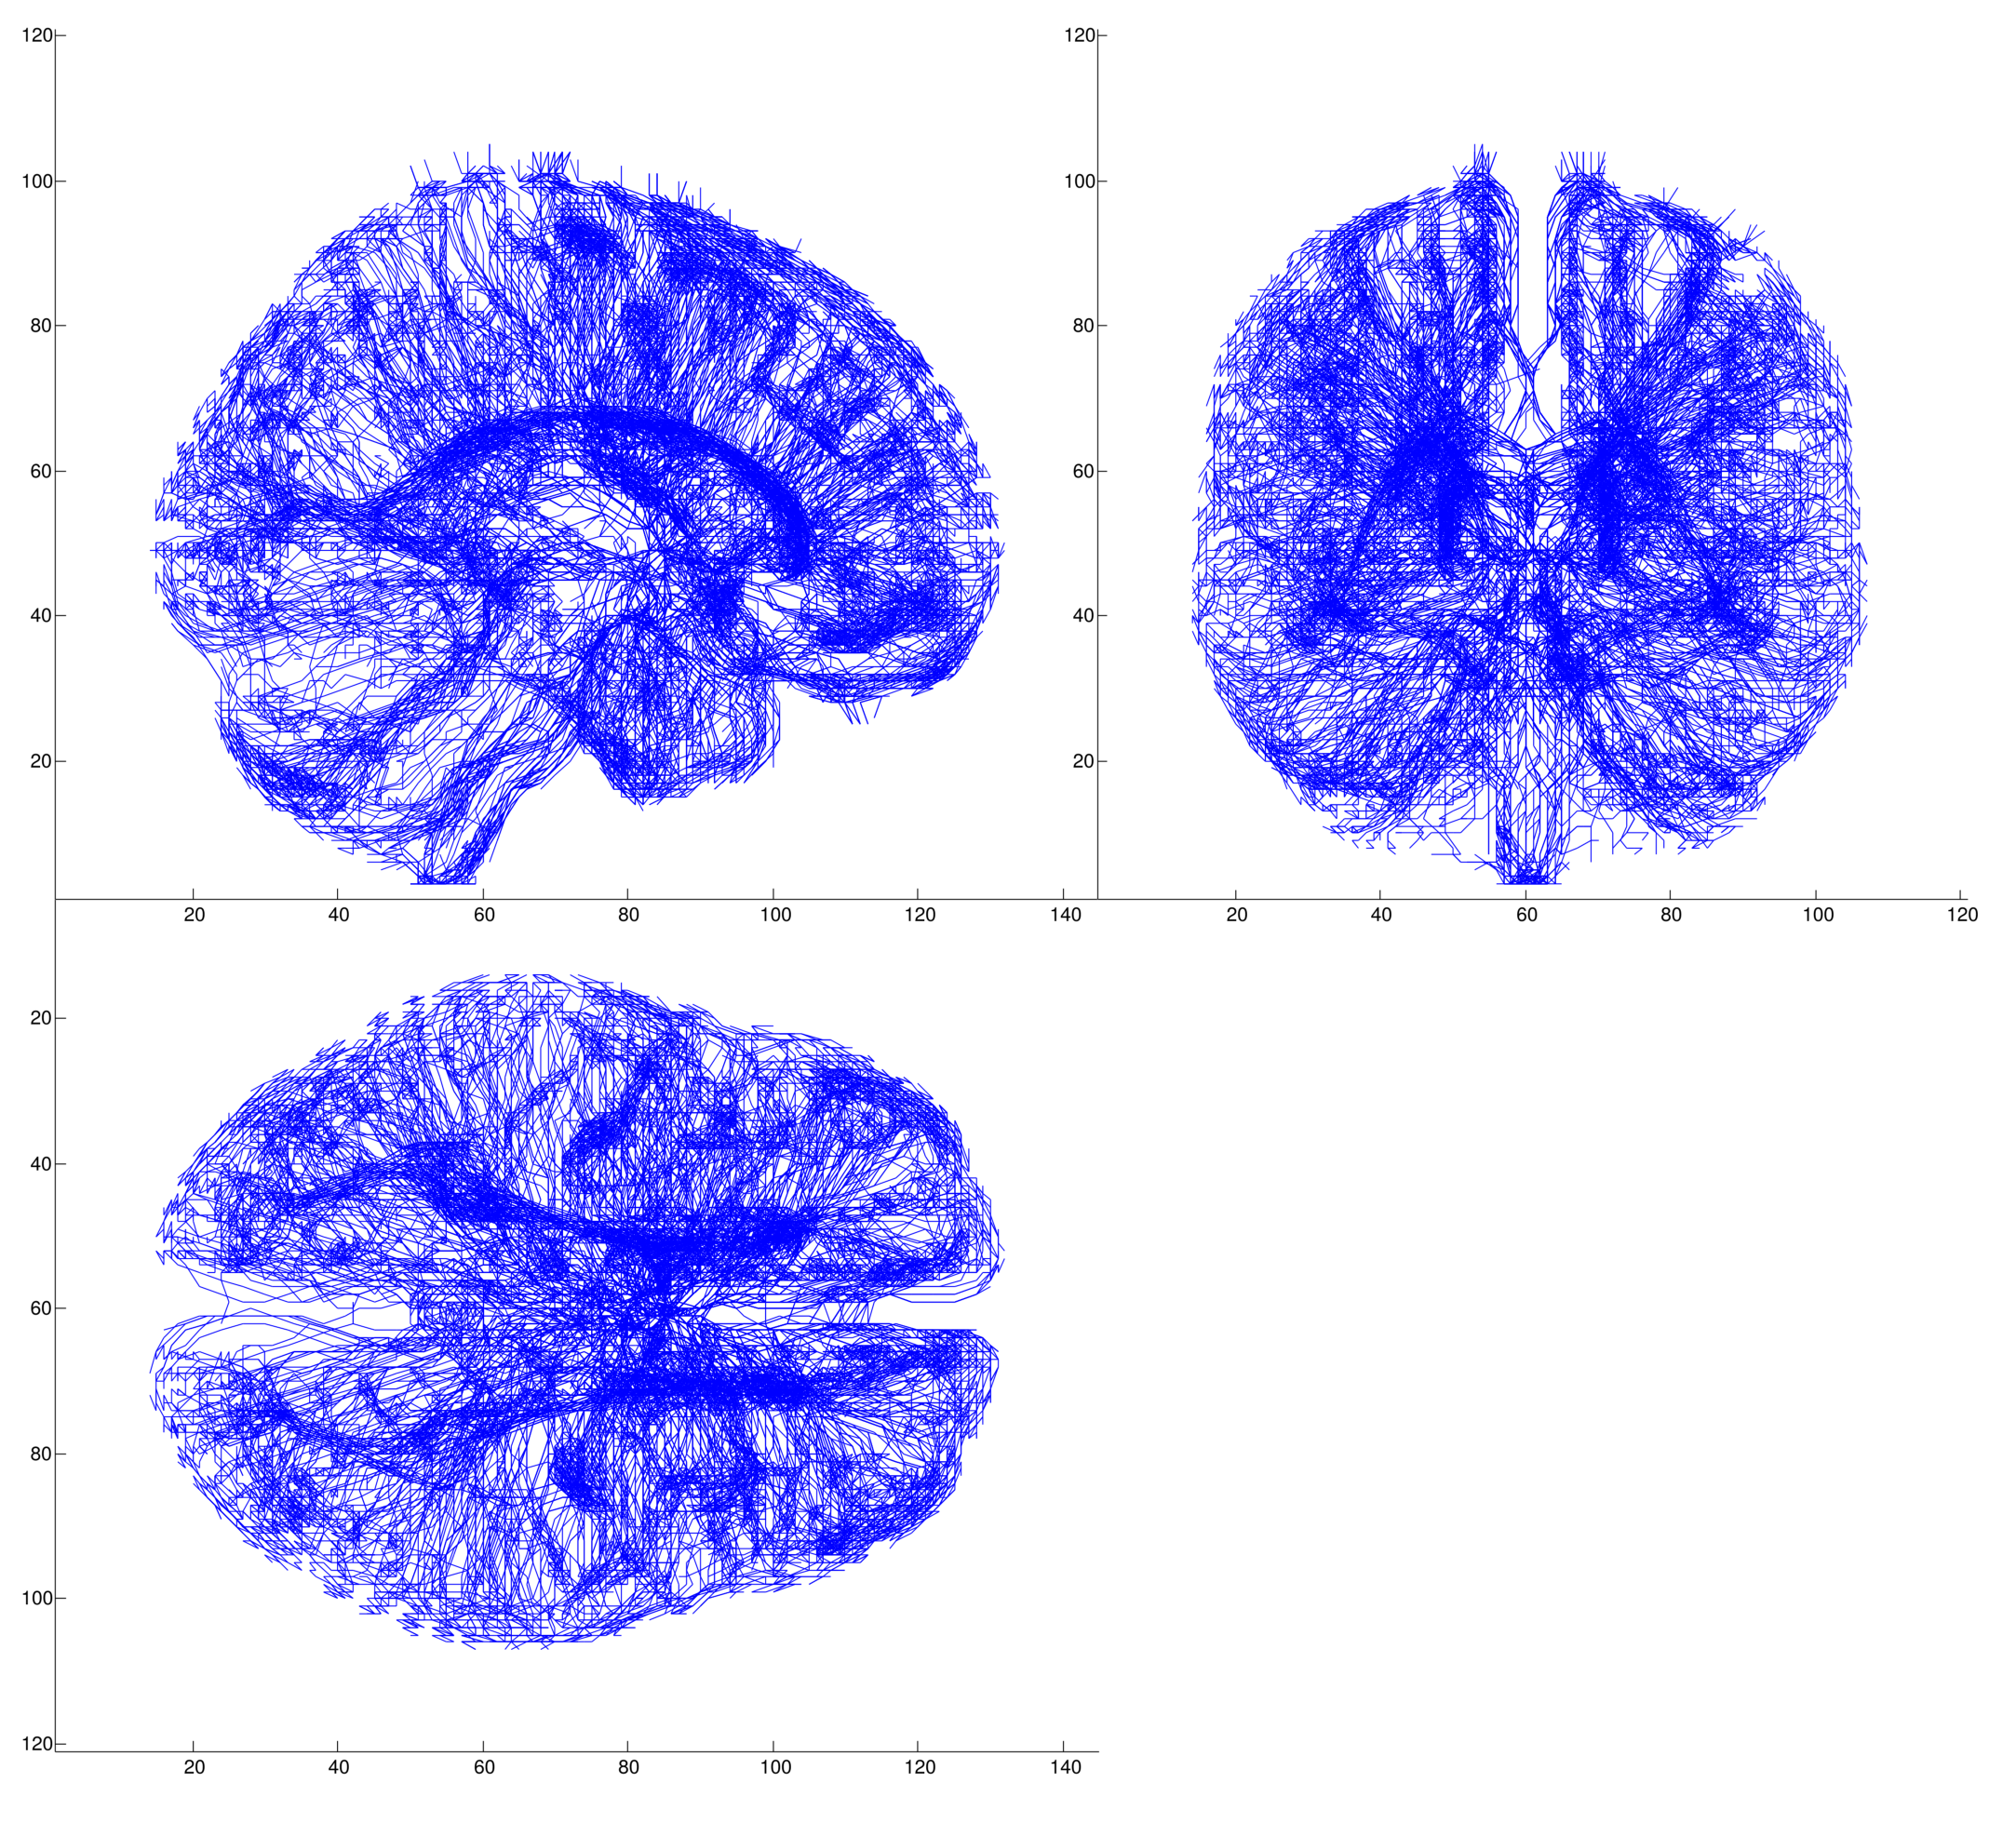
\includegraphics[width=0.7\textwidth]{Graphics/ch6/cuts}
		\caption[Set of \acs{HMM} based paths over the \acs{MRI} DARTEL template.]{Set of \ac{HMM} based paths over the \acs{MRI} DARTEL template.}
		\label{fig:cuts}
	\end{center}
\end{figure}


% Con o sin suavizado
\subsection{Radial Texture Features}\label{sec:rtextfeat}
The paths $\mathbb{P}_{\theta,\varphi}$ proposed above could theoretically be used as a feature selection tool to extract the set of intensities $V_{\theta,\varphi}$ as in the standard \ac{SBM}, and even create hybrid \ac{HMM}-\ac{SBM} maps from that set. However, since these new paths contain geometric information, they encode the internal structure, which is itself an additional feature. This encoding could be used to characterize the texture in the neighbourhood of $\mathbb{P}_{\theta,\varphi}$. 

In \cite{Martinez-MurciaVRLBP} a helical sampling was proposed to define the neighbourhood of the mapping vector $\mathbf{v}_{\theta,\varphi}$. That is infeasible in this case, due to the topology of the \ac{HMM} paths. Conversely, we propose a modification of the \ac{GLCM} (see Section~\ref{sec:haralick}) that instead of computing the texture in a given direction, characterizes it along the defined \ac{HMM} paths. 

This is basically a node-wise \ac{GLCM}, in which the number of grey-level transitions between adjacent nodes, which we could note as $\mathbf{p}_i$ and $\mathbf{p}_{i+1}$, is stored along the whole path $\mathbb{P}_{\theta,\varphi} = \{\mathbf{p}_0, \mathbf{p}_1 \dots \mathbf{p}_N\}$. Mathematically, the computation of the GLCM in each point in the path will be: 
\begin{equation}\label{eq:glcm}
\mathbf{C}_{\Delta_n}(i,j) = \sum_{n=0}^{N-1}
\begin{cases}
1 & I(\mathbf{p}_n) = i, I(\mathbf{p}_{n+1})=j\\
0 & otherwise
\end{cases}
\end{equation}
where the offset is different for each pair of nodes $\Delta_i=\mathbf{p}_{i+1}-\mathbf{p}_i$. 

The definition in Eq.~\ref{eq:glcm} computes the values at each node, without considering the neighbourhood. We can generalize it to include the surrounding vicinity of the $i$-th node $\mathbf{p}_i$ in the \ac{HMM} path, which we have noted as the set $\mathbb{X}_i$. Under this generalization, equation~\ref{eq:glcm} becomes: 
\begin{equation}\label{eq:glcmGen}
\mathbf{C}(i,j) = \sum_{n=0}^{N-1} \sum_{\mathbf{p} \in \mathbb{X}_i}
\begin{cases}
1 & I(\mathbf{p}) = i, I(\mathbf{p}+\Delta_n)=j\\
0 & otherwise
\end{cases}
\end{equation}

Once the \ac{GLCM} is computed, we can extract a variety of texture descriptors, as defined in Section~\ref{sec:haralickFeatures}. Specifically, in this work, we will use the aforementioned Energy (eq.~\ref{eq:energy}), Entropy (eq.~\ref{eq:entropy}), Correlation (eq.~\ref{eq:correlation}), Contrast (eq.~\ref{eq:contrastHar}) and Homogeneity (eq.~\ref{eq:homogeneity}), along with other texture features proposed in the original Haralick's article \cite{Haralick73} as well as in \cite{soh1999texture} and \cite{clausi2002analysis}. These are Dissimilarity\cite{soh1999texture} (eq.~\ref{eq:dissimilarity}), Difference Variance\cite{Haralick73} (D. Variance, eq~\ref{eq:dvar}), Difference Entropy\cite{Haralick73} (D. Entropy, eq~\ref{eq:dent}), Inverse Difference Normalized\cite{clausi2002analysis} (IDN, eq~\ref{eq:idn}) and Inverse Difference Moment Normalized\cite{clausi2002analysis} (IDMN, eq.~\ref{eq:idmn}). 

\begin{align}\label{eq:dissimilarity}
\text{Dissimilarity} & = \sum_i\sum_j\{|i-j|\mathbf{P}(i,j)\}\\\label{eq:dvar}
\text{D. Variance} &=  \text{VAR}\left\lbrace\sum_{|i-j|=k}\mathbf{P}(i,j)\right\rbrace\\\label{eq:dent}
\text{D. Entropy} &= -\sum\limits_{k=0}^{N_g-1} \sum_{|i-j|=k}\mathbf{P}(i,j) \log \left\lbrace \sum_{|i-j|=k}\mathbf{P}(i,j)\right\rbrace \\\label{eq:idn}
\text{IDN} &= \sum_i\sum_j \frac{\mathbf{P}(i,j)}{1+|i-j|/N}\\ \label{eq:idmn}
\text{IDMN} &= \sum_i\sum_j \frac{\mathbf{P}(i,j)}{i+(j-j)^2/N^2}
\end{align}

\section{Evaluation}
In this chapter, we have proposed a completely new framework for extracting features and visualizing structural \ac{MRI} images from the \adnimri{} database. To evaluate them, we will combine statistical significance assessment and classification analysis. For this purpose, we propose the following experiments: 
\begin{itemize}
	\item Experiment 1: assessment of the original \ac{SBM} maps and the \ac{VRLBP} over segmented \ac{GM} and \ac{WM} images. We will provide a statistical significance analysis and a classification analysis under the \ac{AD} vs \ac{CTL} scenario of the six proposed maps. 
	\item Experiment 2: assessment of the layered extension of the \ac{SBM} over segmented \ac{GM} and \ac{WM} images. That way, we want to prove if dividing the sampling set, and thus, increasing the depth resolution of the system affects the overall performance of our system. We will provide statistical significance analysis and classification analysis under the \ac{AD} vs \ac{CTL} scenario . 
	\item Experiment 3: evaluation of the \ac{HMM} based paths on simulated datasets, to demonstrate the ability of this algorithm to adapt to different intensity distributions. 
	\item Experiment 4: evaluation of the \ac{HMM} based paths on a real \ac{MRI} dataset, by taking the different paths as feature selectors, and evaluating the performance obtained by the set of intensities selected by each individual path, a combination of them, and the further construction of hybrid \ac{HMM}-\ac{SBM} maps. We provide a classification analysis of the selected features under the \ac{AD} vs \ac{CTL} scenario. 
	\item Experiment 5: evaluation of the texture maps derived from the \ac{HMM} based paths on the T1-weighted \ac{MRI} dataset, under a classification analysis of \ac{AD} vs \ac{CTL} subjects. 
\end{itemize}

In te first three experiments, we will used segmented \ac{GM} and \ac{WM} maps, where in experiments 5 and 6, we will use raw, T1-weighted images. The classification analysis is performed by using a linear \ac{SVC} for classifying, and 10-fold cross validation strategy (see Section~\ref{sec:validation} for more details). For estimating statistical significance, we use the two-sample $t$-test defined in Section~\ref{sec:ttestEq}. 


\section{Results}

\subsection{Experiment 1: Original and \acs{VRLBP} Spherical Brain Mapping}
First, with experiment 1, we test the original and \ac{VRLBP} \ac{SBM} maps, by means of significance and classification analysis. To start with, we provide the significance maps computed under the \ac{AD} vs \ac{CTL} scenario in the six original \ac{SBM} measures (surface, thickness, number of folds, average, entropy and kurtosis) in  Figure~\ref{fig:tmaps}. 

\begin{figure*}[htp]
	\centering
	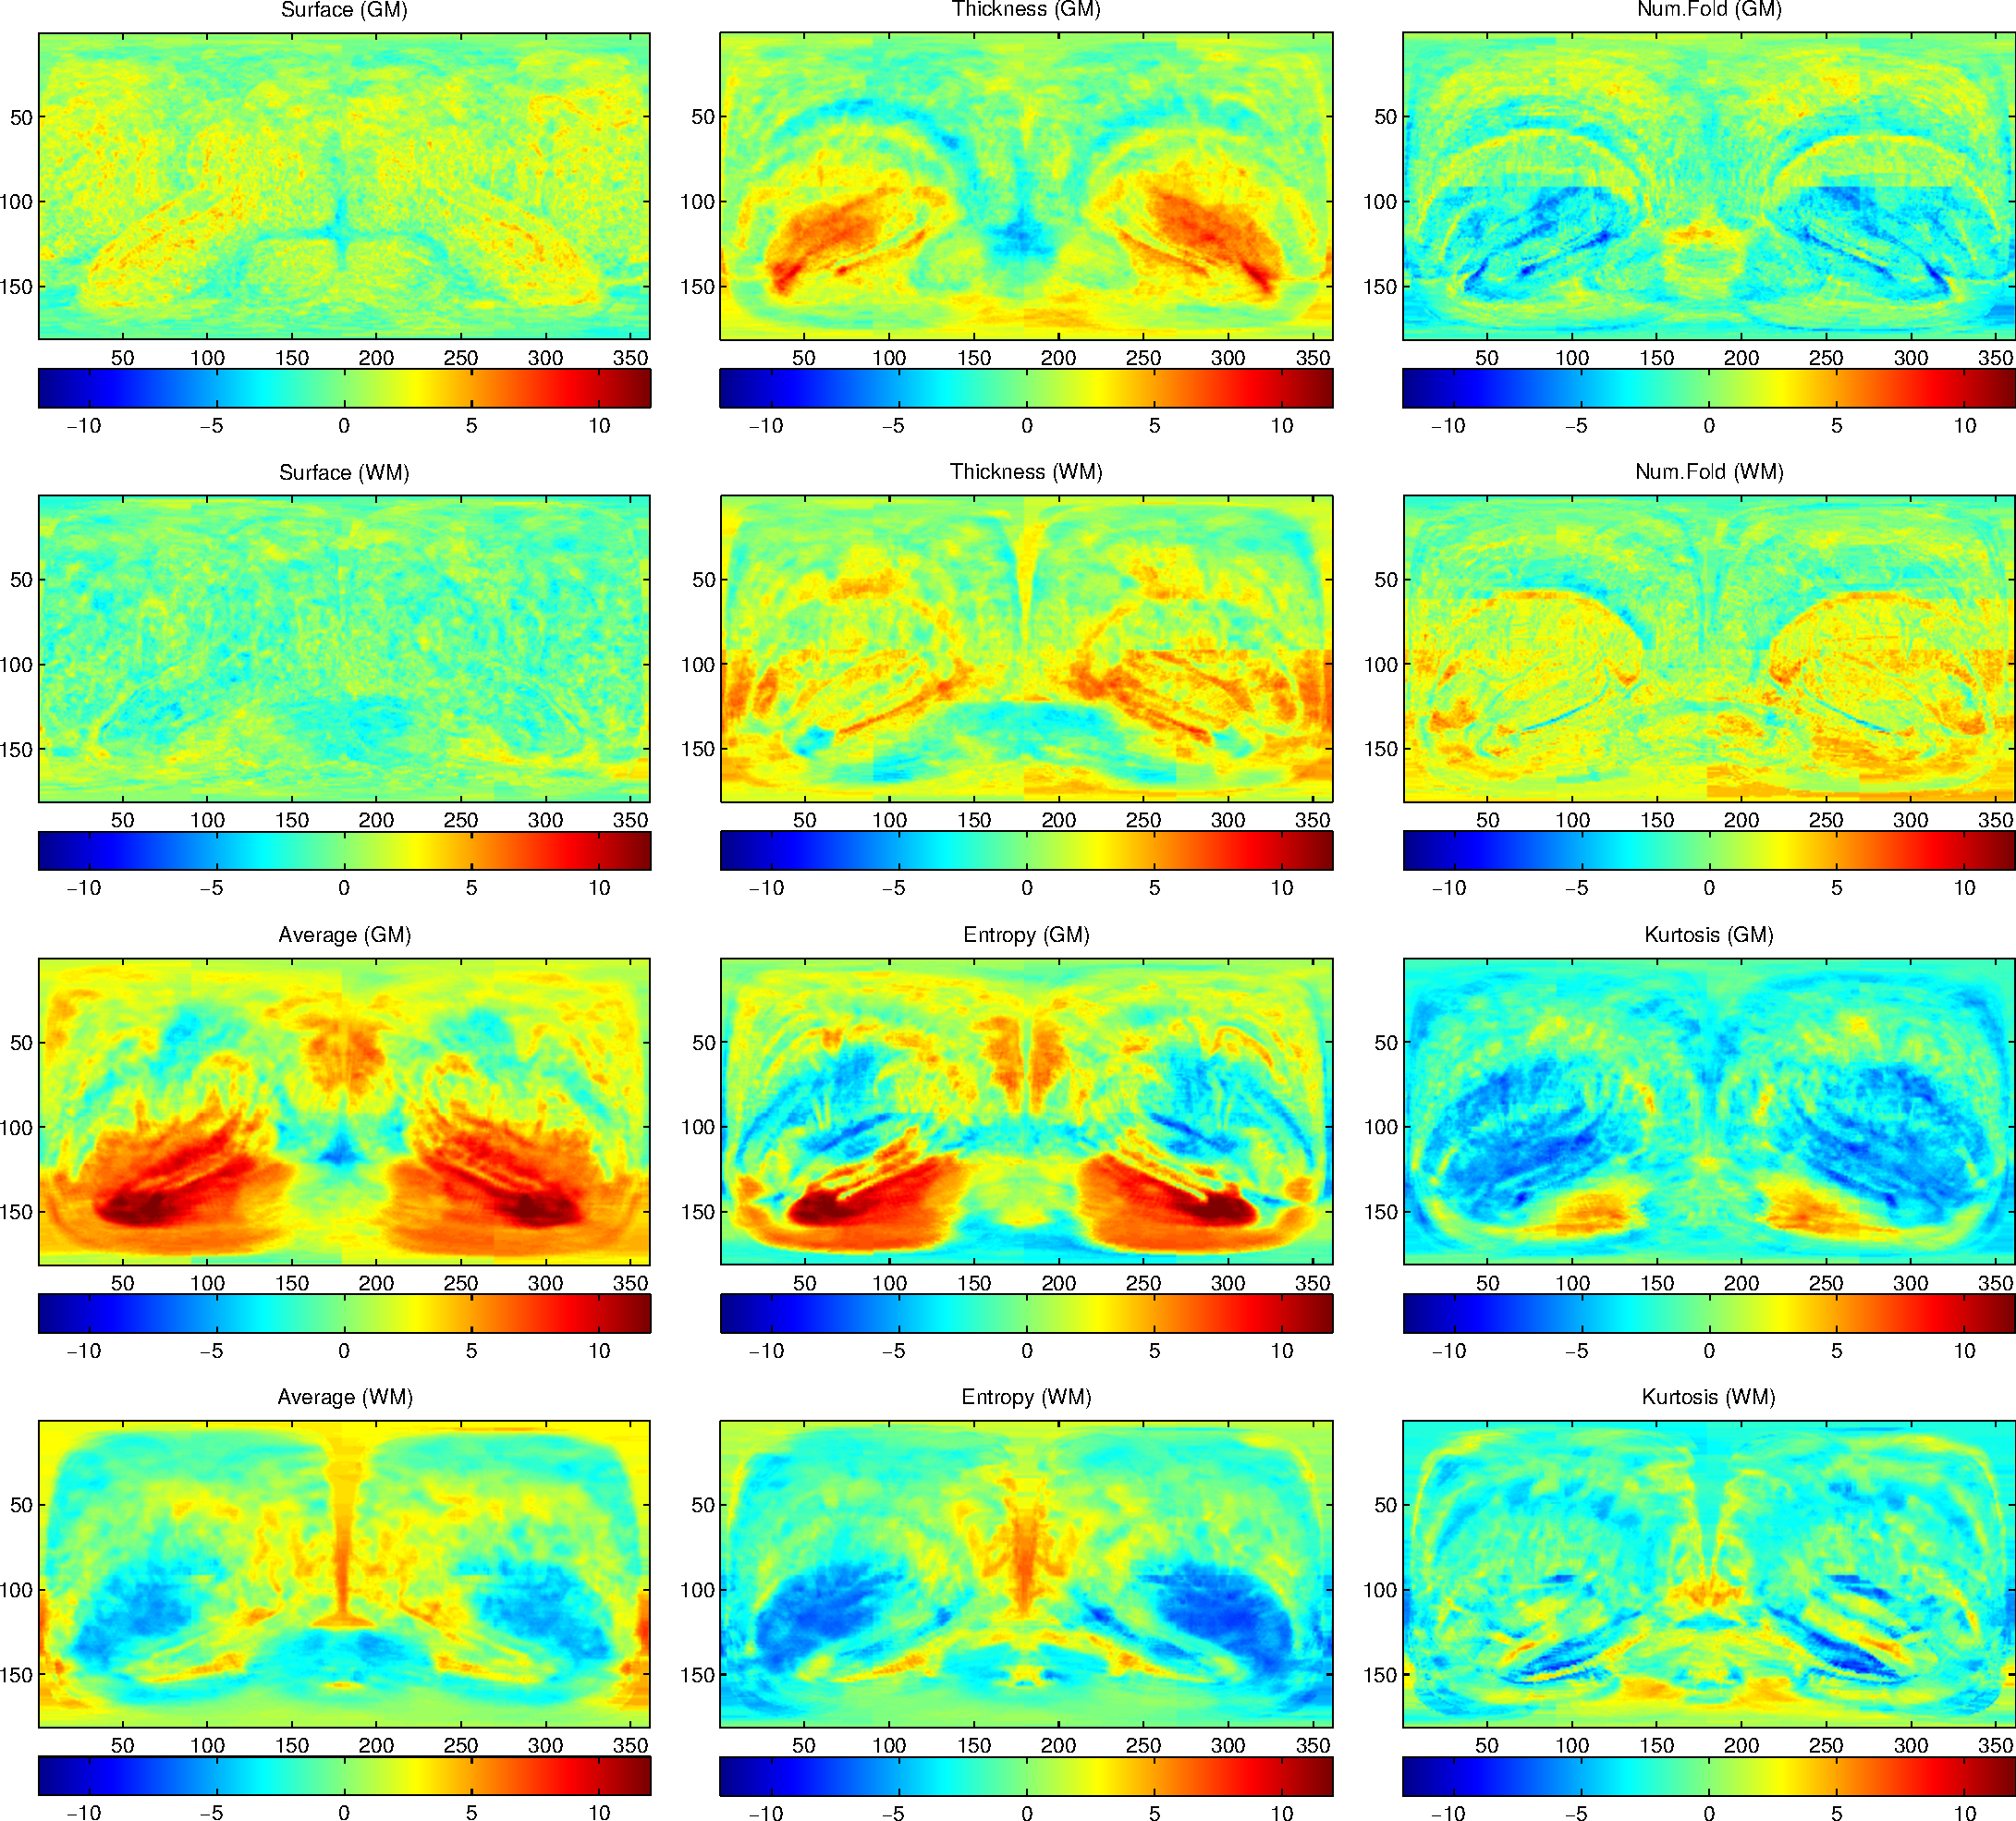
\includegraphics[width=0.9\textwidth]{Graphics/ch6/07-tmaps}
	\caption[\acs{SBM} t-maps under the \acs{AD} vs \acs{CTL} for \acs{GM} and \acs{WM} images.]{$t$-maps to assess the regions with a higher statistical relevance in the \acs{AD} vs \acs{CTL} paradigm, for each \ac{SBM} measure and using \ac{GM} and \ac{WM} maps. }
	\label{fig:tmaps}
\end{figure*}

For $p<0.05$, in the database subset of the \adnimri{}, the signifcance threshold can be established at $|t|>1.96$. This means that, in Figure~\ref{fig:tmaps}, the most relevant differences between classes can be found at the areas coloured in dark red (positive, \ac{CTL} subjects have a higher measure) and dark blue (negative, \ac{AD} subjects have a higher measure). For the anatomic structures, we refer to the anatomical reference presented in Section~\ref{sec:anatomical}. 

We first note that the surface measure, tested in both \ac{GM} and \ac{WM} maps, does not look relevant. Very few significant pixels are scattered throughout the image, although with a slightly higher concentration in the areas corresponding to the temporal lobe. 

In the remaining \ac{GM} maps, we observe similar behaviours, with higher absolute $t$-values located in the frontal, occipital and parietal lobes. But again, the most significant areas can be found at the temporal lobe. It is more obvious in the average and entropy measures, but can also be found at the thickness, or negatively in the number of folds and kurtosis maps. This points to the well kown fact that most of the neurodegeneration in \ac{GM} occurs within the structures that are mapped to these directions, including mid temporal lobe, amygdala, hippocampus or parahippocampal gyrus, considered a strong indicator in the NINCDS-ADRDA criteria \cite{Dubois2007}. Other \ac{GM} structures such as the caudate nucleus and putamen also appear with significant $t$ values, especially in the entropy and kurtosis maps (with negative $t$) \cite{Pievani2013}. 

In the \ac{WM}, the levels of significance achieved are smaller than in the \ac{GM}, but still high. We see the higher levels of number of folds and thickness located in the vicinity of those obtained for \ac{GM}, but in negative. For the average, entropy and kurtosis measures, we observe a different behaviours. These maps present large areas of negative $t$-values located in the Caudate Nucleus, Globus Pallidus and Putamen. Areas around the posterior cingulate gyrus and the adjacent precuneus also present reduced $t$ values, which could be related to cell loss, as suggested in \cite{Baron2001}.

\begin{figure*}[htp]
	\centering
	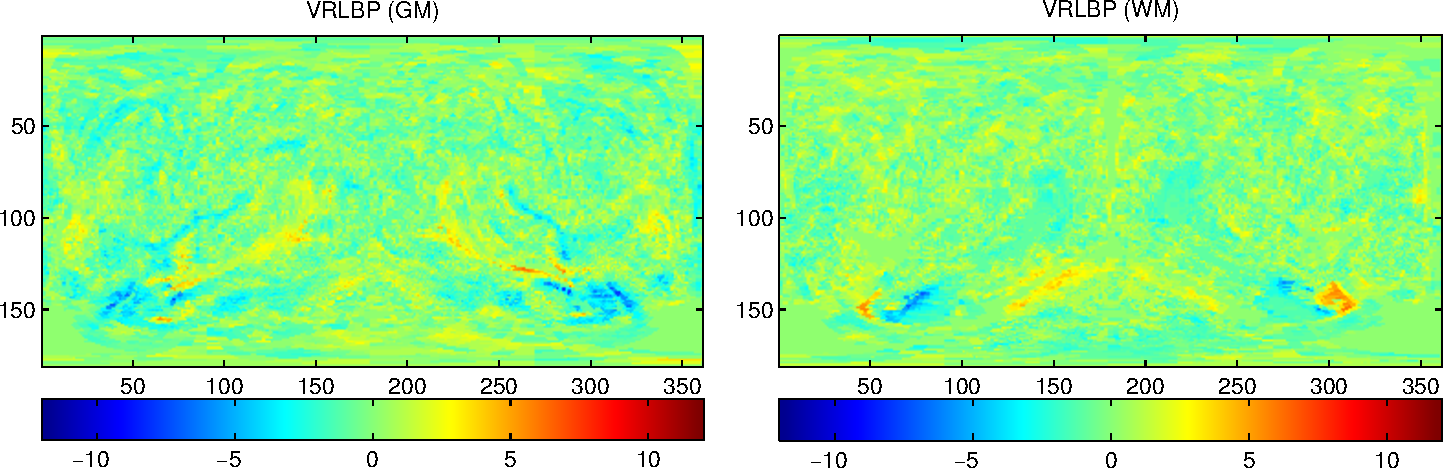
\includegraphics[width=\textwidth]{Graphics/ch6/09-tmaps_vrlbp}
	\caption[$t$-maps for the \acs{VRLBP}-\acs{SBM} in the \acs{AD} vs \acs{CTL} scenario.]{Maps that present the level of the $t$ statistic in the \ac{AD} vs. \ac{CTL} paradigm, for the VRLBP projections mapping over a) \ac{GM} and b) \ac{WM}. }
	\label{fig:tmapvrlbp}
\end{figure*}

Finally, we take a look at the statistical significance of the \ac{VRLBP} maps. In Figure~\ref{fig:tmapvrlbp}, we can observe that most of the image features small $t$ values, however there are small areas that contain higher significance. These areas correspond to the temporal lobe, amygdala and hippocampus (in the \ac{GM} maps) and smaller regions located at the limits between the hippocampus and amygdala (in \ac{WM}).

Now, we perform a classification analysis of the images. To this purpose, we will use the computed $t$-maps to select the most relevant pixels in the \ac{SBM} maps, which will be used to train and test a \ac{SVC}. The performance results for the six original measures and the \ac{VRLBP} approach, including the percentage of selected pixels (perc.), can be found at Table~\ref{tab:perfProj}. 

\begin{table*}[htp]
	\myfloatalign
	\begin{tabularx}{\textwidth}{Xcccc}
		\toprule
		\tableheadline{Approach} & \tableheadline{Perc.} & \tableheadline{Accuracy} & \tableheadline{Sensitivity} & \tableheadline{Specificity}\\
		\midrule
		Surface (\ac{GM}) & $0.100$ & $0.638 \pm 0.006$ & $0.660 \pm 0.030$ & $0.616 \pm 0.024$ \\
		Surface (\ac{WM}) & $0.100$ & $0.672 \pm 0.007$ & $0.692 \pm 0.018$ & $0.652 \pm 0.018$ \\
		\midrule
		Thickness (\ac{GM})  & $0.725$ & $0.781 \pm 0.007$ & $0.811 \pm 0.011$ & $0.751 \pm 0.017$ \\
		Thickness (\ac{WM}) & $0.925$ & $0.758 \pm 0.009$ & $0.773 \pm 0.017$ & $0.744 \pm 0.011$ \\
		\midrule
		Num.Fold (\ac{GM}) & $0.600$ & $0.749 \pm 0.013$ & $0.782 \pm 0.019$ & $0.716 \pm 0.013$ \\
		Num.Fold (\ac{WM}) & $0.500$ & $0.757 \pm 0.005$ & $0.745 \pm 0.006$ & $0.768 \pm 0.009$ \\
		\midrule
		Average (\ac{GM}) & $0.575$ & $0.879 \pm 0.005$ & $0.897 \pm 0.006$ & $0.861 \pm 0.006$ \\
		Average (\ac{WM}) & $0.150$ & $0.800 \pm 0.011$ & $0.802 \pm 0.013$ & $0.798 \pm 0.009$ \\
		\midrule
		Entropy (\ac{GM}) & $0.825$ & $0.846 \pm 0.008$ & $0.842 \pm 0.009$ & $0.849 \pm 0.011$ \\
		Entropy (\ac{WM}) & $0.525$ & $0.796 \pm 0.006$ & $0.811 \pm 0.009$ & $0.781 \pm 0.009$ \\
		\midrule
		Kurtosis (\ac{GM}) & $1.000$ & $0.753 \pm 0.007$ & $0.801 \pm 0.011$ & $0.704 \pm 0.015$ \\
		Kurtosis (\ac{WM}) & $0.175$ & $0.697 \pm 0.008$ & $0.702 \pm 0.018$ & $0.693 \pm 0.009$ \\
		\midrule
		VRLBP (\ac{GM}) & $0.200$ & $0.903 \pm 0.010$ & $0.890 \pm 0.012$ & $0.916 \pm 0.018$ \\
		VRLBP (\ac{WM}) & $0.150$ & $0.909 \pm 0.014$ & $0.899 \pm 0.028$ & $0.919 \pm 0.018$ \\
		\bottomrule
	\end{tabularx}
	\caption{Performance values (Average $\pm$ Standard Deviation) for the different \ac{SBM} approaches.}
	\label{tab:perfProj}
\end{table*}

We can see a general trend in which the statistical measures (average, entropy and kurtosis) clearly outperform the morphological ones (surface, thickness and number of folds), although the tissue thickness is the best performing of these, as it could be expected. For \ac{GM} maps, average ($0.879 \pm 0.005$) and entropy ($0.846 \pm 0.008$) achieve the best perforance, followed by thickness ($0.781 \pm 0.007$), kurtosis ($0.753 \pm 0.019$), and finally, the number of folds ($0.749 \pm 0.013$) and surface ($0.638 \pm 0.006$). These results match what we presented previously with the statistical maps, in which the surface contained the less significant measures. 

As for the performance of the \ac{SBM} measures based on \ac{WM} maps, the rank is very similar to that obtained for \ac{GM}. Again, average ($0.800 \pm 0.011$) and entropy ($0.796 \pm 0.006$) are the best performing features among the original measures. They are followed by thickness and the number of folds, with respectively $0.758 \pm 0.009$ and $0.757 \pm 0.005$. Finally, the kurtosis and the surface are the less discriminant measures again, with $0.697 \pm 0.008$ and $0.672 \pm 0.007$. All these measures are outperformed by the \ac{VRLBP} approach, which achieves more than 90\% accuracy in both \ac{GM} and \ac{WM}. 

\begin{figure*}[htp]
	\centering
	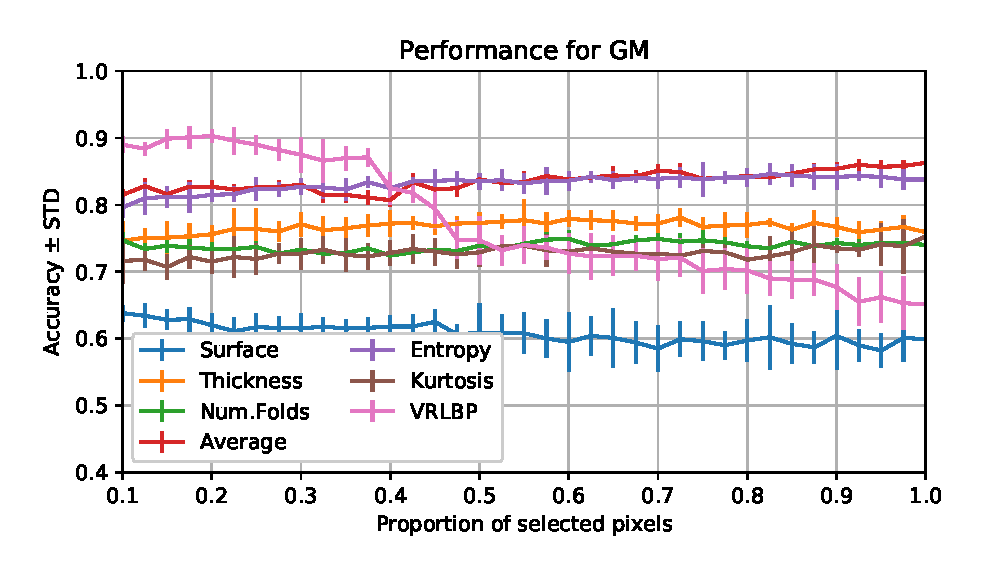
\includegraphics[width=0.9\textwidth]{Graphics/ch6/GMperformanceComp}\\
	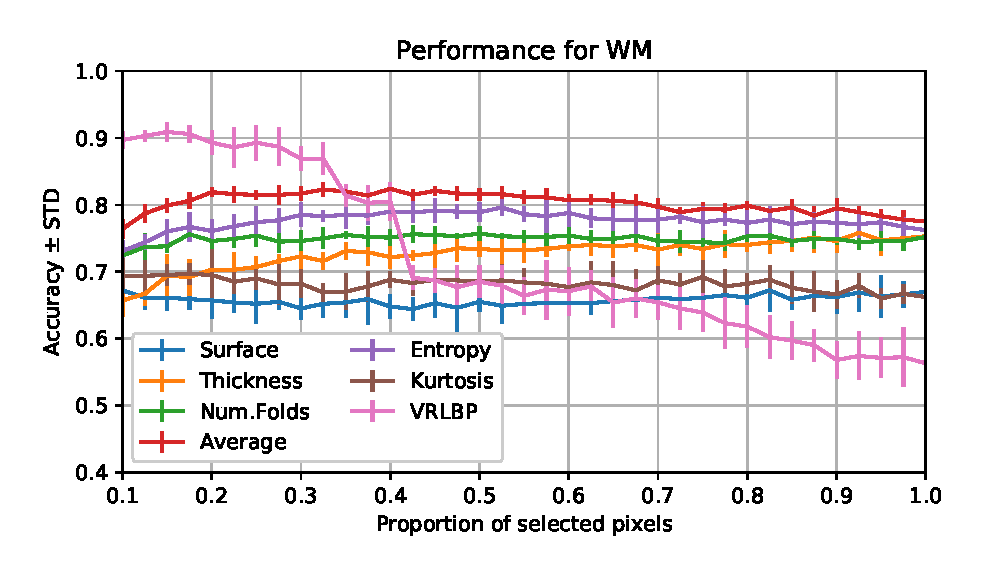
\includegraphics[width=0.9\textwidth]{Graphics/ch6/WMperformanceComp}
	\caption{Performance for the different \ac{SBM} approaches over the: a) \acs{GM} and b) \acs{WM}.}
	\label{fig:figureGM}
\end{figure*}

In Figure~\ref{fig:figureGM} we explore the evolution of the performance as the number of selected pixels varies. Very small differences in the accuracy exist for most measures, and so, we can consider that the performance of the \ac{SBM}, once that a few thousand significant pixels (a 10\% of $181\times361=65341$) have been selected, the system performs well independently of that number. That is, however, not the case of the surface approach, and more remarkably, of the \ac{VRLBP}. In this latter case, for both tissues, the performance is high in the first 40\% of selected voxels, but after that, it dramatically decreases down to less than 70\% accuracy. 

\subsection{Experiment 2: Layered Extension}\label{sec:layeredttest}
In Experiment 2, we have assessed how the performance of our \ac{SBM} varies when adding different layers, which could theoretically improve the accuracy of the \ac{SBM} representation. First, we will take a look at the performance achieved by this extension on all six original \ac{SBM} maps, using 4 layers and different $t$-thresholds (2, 4, 8 and 10). This is presented at Figure~\ref{fig:layeredPerf}. 

\begin{figure*}[htp]
	\centering
	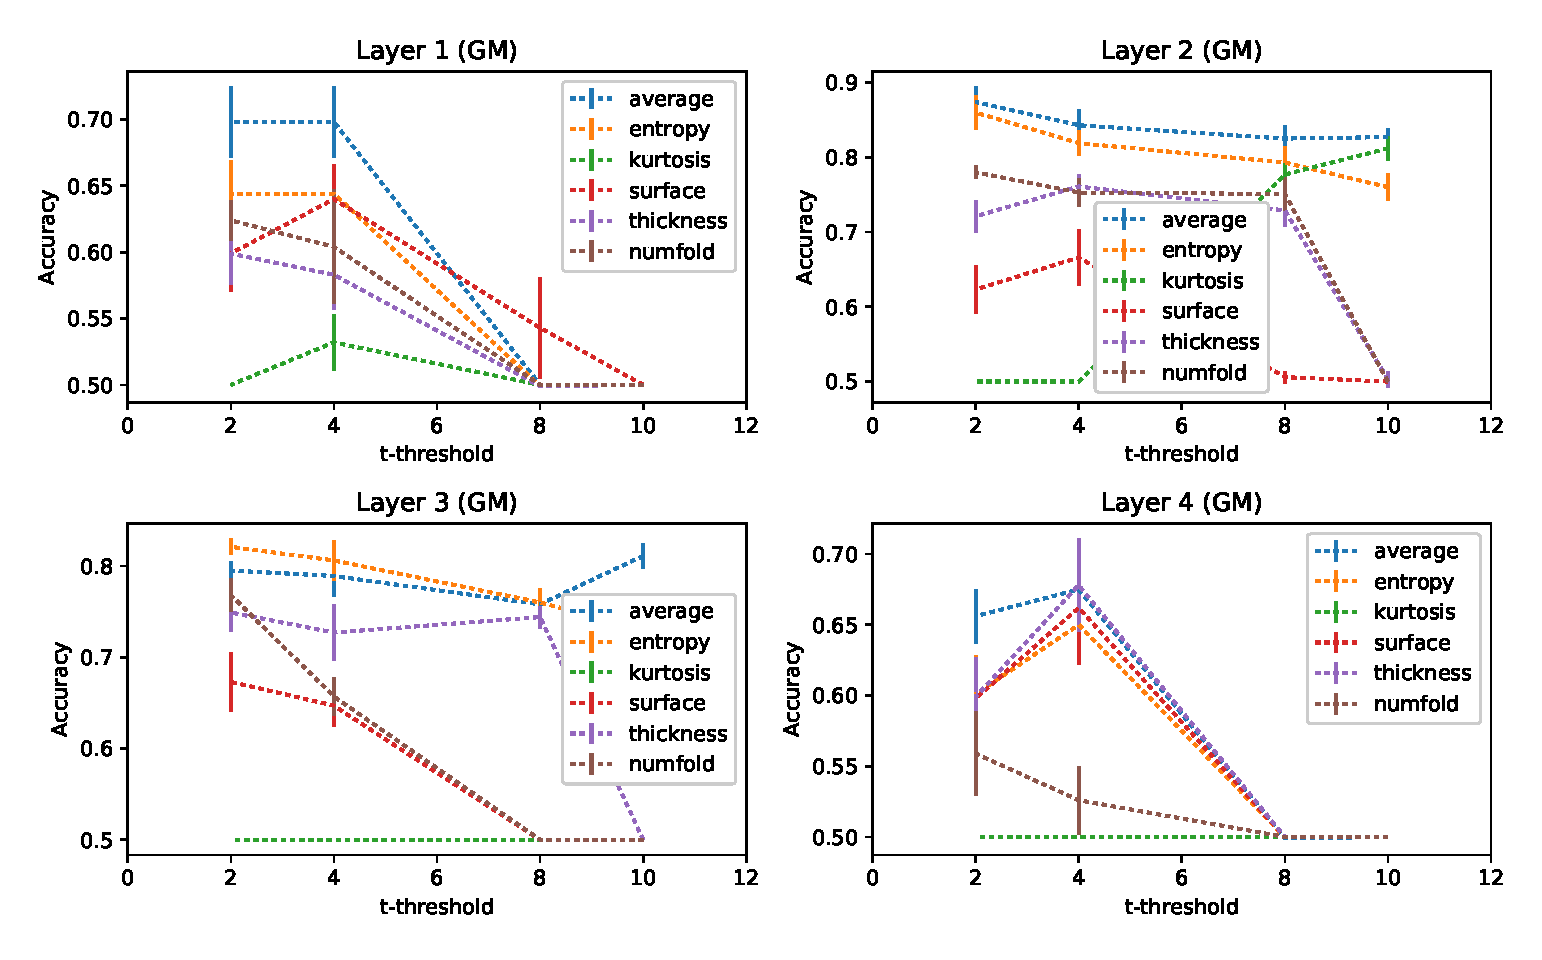
\includegraphics[width=0.9\textwidth]{Graphics/ch6/layerPerfGM}\\
	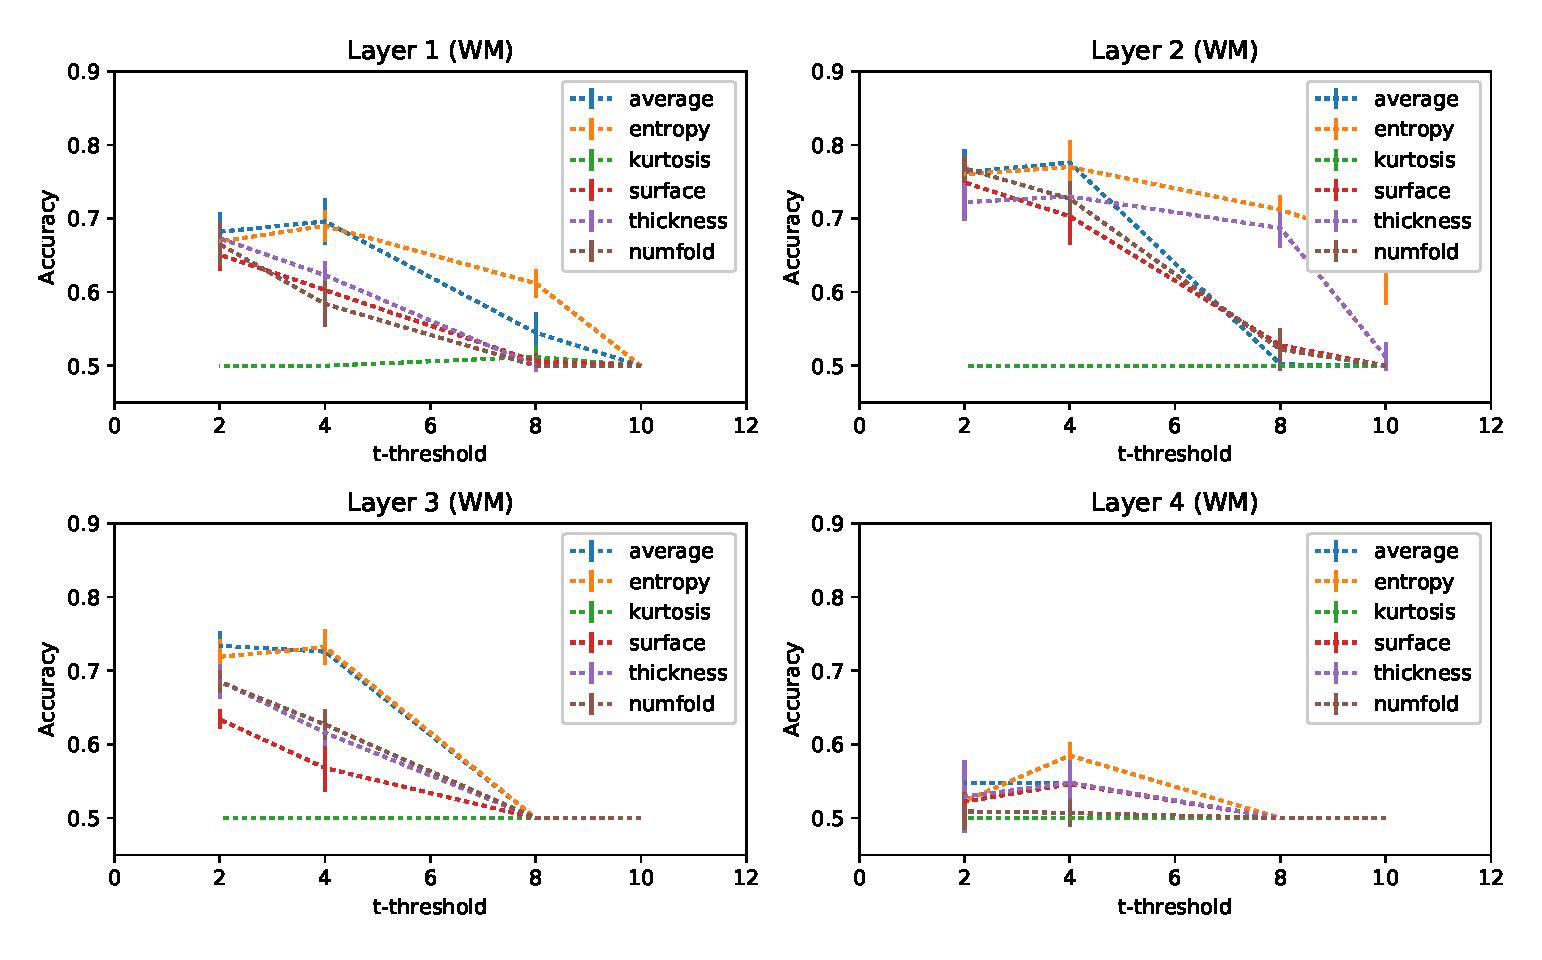
\includegraphics[width=0.9\textwidth]{Graphics/ch6/layerPerfWM}
	
	\caption[Performance of the four-layered mappings.]{Performance for the different four-layered mappings over the: a) \acs{GM} and b) \acs{WM} at different levels of statistical significance.}
	\label{fig:layeredPerf}
\end{figure*}

The first thing that we can observe is that for \ac{GM} maps, the better performance is achieved within the second and third layers, and only for the second layer in the case of \ac{WM}. In almost all cases, the average performance achieves higher accuracy than any other \ac{SBM} measure, closely followed by entropy. It also tells us that, with less restrictive $t$-thresholds, the performance generally decreases, and the best values are between 2 and 4. 

Performing a significance analysis on the 4 layer extension of the 7 proposed \ac{SBM} maps over the \ac{GM} and \ac{WM} images could be infeasible for this thesis, therefore we will only provide $t$-maps of the best performing measure: the average on the \ac{GM} and \ac{WM} tissues. The significance assessing of this case is found at Figure~\ref{fig:tmaplayered}.

\begin{figure*}[htp]
	\centering
	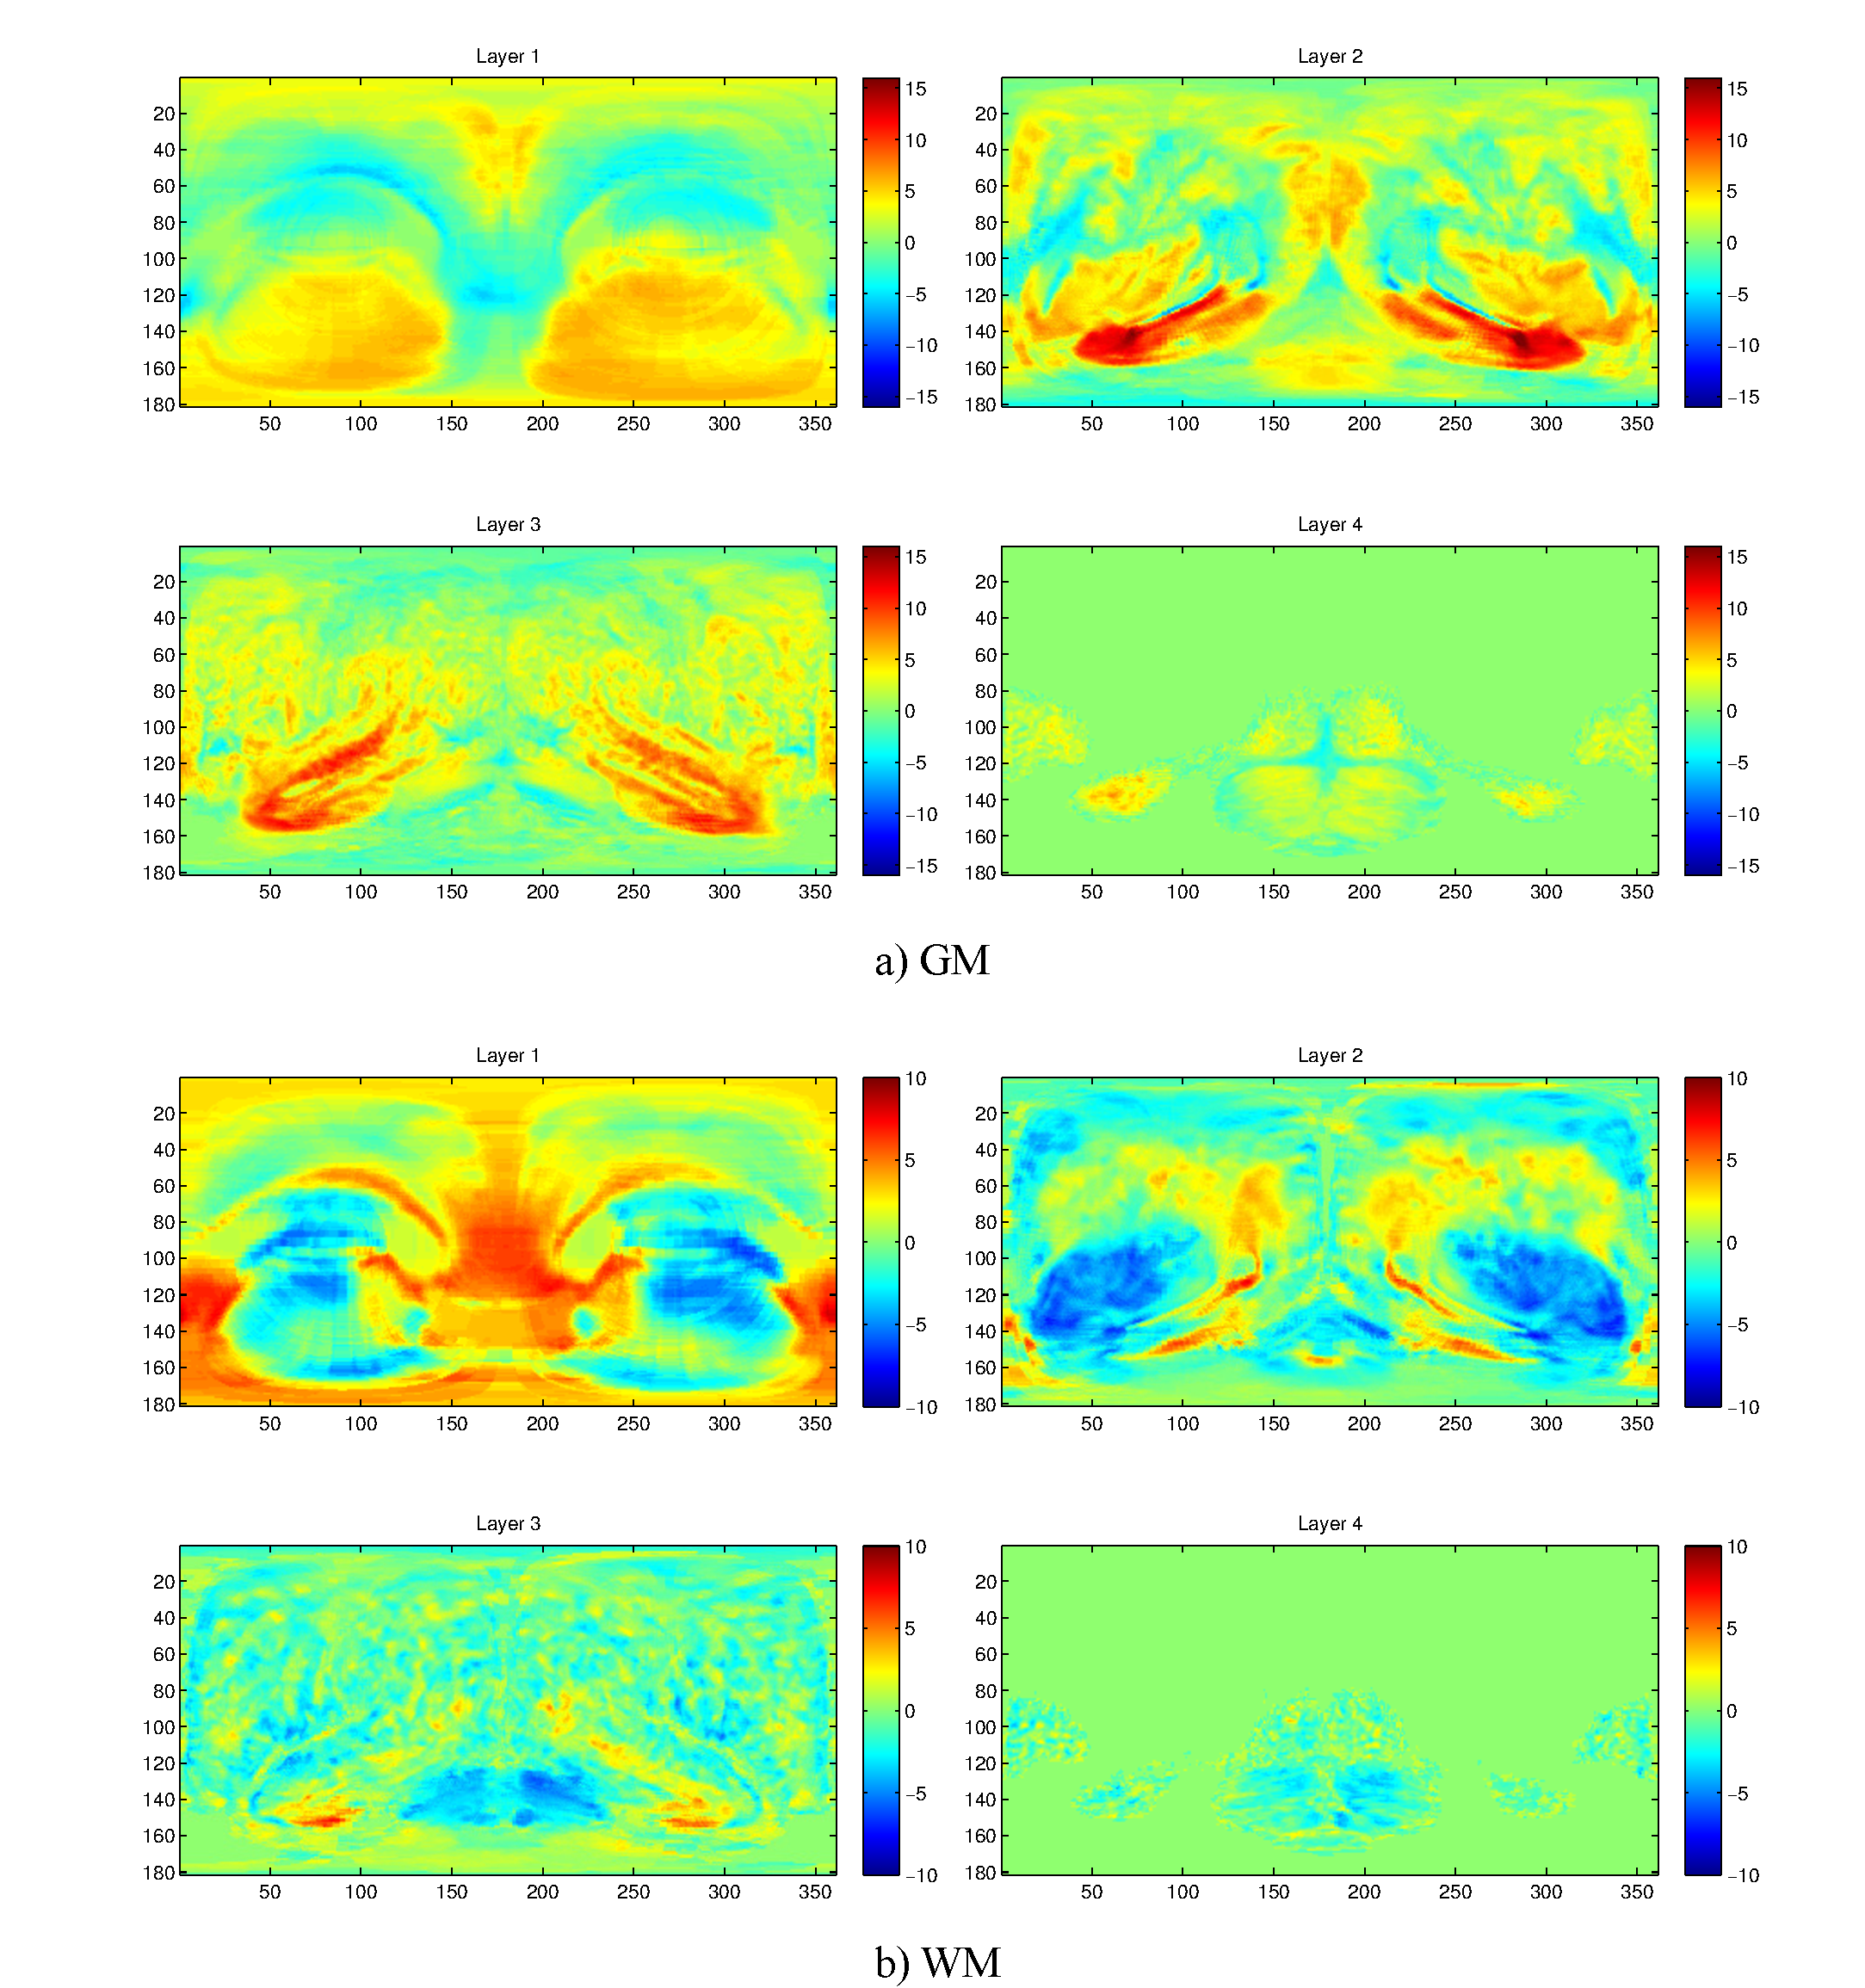
\includegraphics[width=\textwidth]{Graphics/ch6/08-Tmap4LayAverage}
	\caption[$t$-maps that present the level of statistical relevance in the \acs{AD} vs \acs{CTL} paradigm.]{$t$-maps that present the level of statistical relevance in the \acs{AD} vs \acs{CTL} paradigm, for a four-layered average mapping over a) \ac{GM} and b) \ac{WM}. }
	\label{fig:tmaplayered}
\end{figure*} 

In \ac{GM}, the most obvious changes are located in layers 2 and 3, specifically at the hippocampus, parahippocampal gyrus and amygdala (layer 2), and the temporal lobe (layer 3), where the values achieved by \ac{CTL} subjects are much higher than those found in \ac{AD}. This could reveal atrophy in these organs, as it has been reported in the literature \cite{Dubois2007,Pievani2013} and will be discussed later. For \ac{WM}, we obtain large negative $t$-values in areas occupied by the rolandic operculum, heschl's gyri, putamen and globus pallidus, with positive values in parts of the hippocampus, and parts of the temporal lobe. Nevertheless, the most significant differences can be located in layer 1, at the borders between ventricles and thalamus, and the cuneus, precuneus and posterior cingulate gyrus, which have been reported in \cite{Baron2001}.

\subsection{Experiment 3: \acs{HMM} on Synthetic Datasets}

\begin{figure}
	\begin{center}
		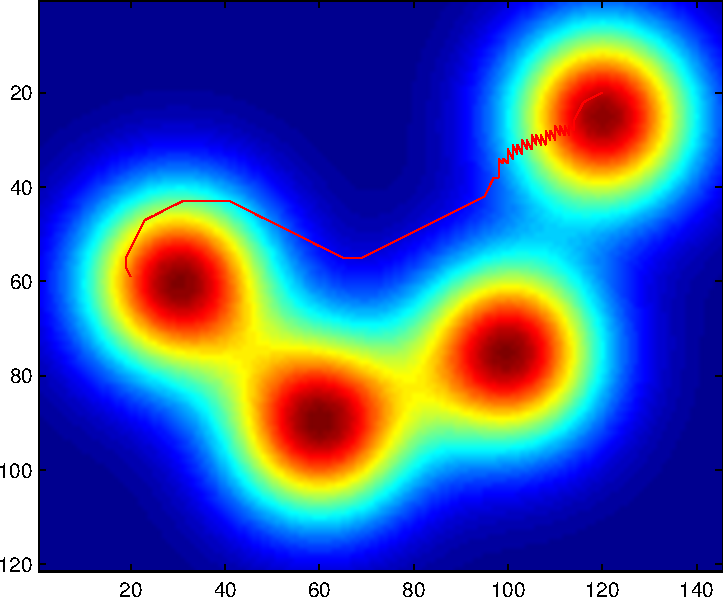
\includegraphics[width=0.5\textwidth]{Graphics/ch6/gaussian}
		\caption{Path traced over a gaussian mixture distribution of 4 i\-so\-tro\-pic gaussian kernels.}
		\label{fig:gaussian}
	\end{center}
\end{figure}

Now, we will analyse the behaviour of the \ac{HMM} paths on some examples. In Figure~\ref{fig:gaussian}, we used a gaussian mixture probability density function, with four isotropic gaussian kernel, to generate a synthetic image. We wanted to test the direction of the \ac{HMM} paths on this image, by locating the initial point $\mathbf{p}_0 = (120,20)$ and the attractor at the centre of one of the kernels, $\mathbf{p}_N = (20, 60)$. This simple example illustrates how the generated paths maximizes both the orientation of the path (towards $\mathbf{p}_N$) and the minimum change in the intensity values. This was specially noticeable in the last nodes of the path, where the approximation to $\mathbf{p}_N$ is very gradual, due to the restrictions imposed. In this example, we used a support ball with $r=3$.


\begin{figure}
	\begin{center}
		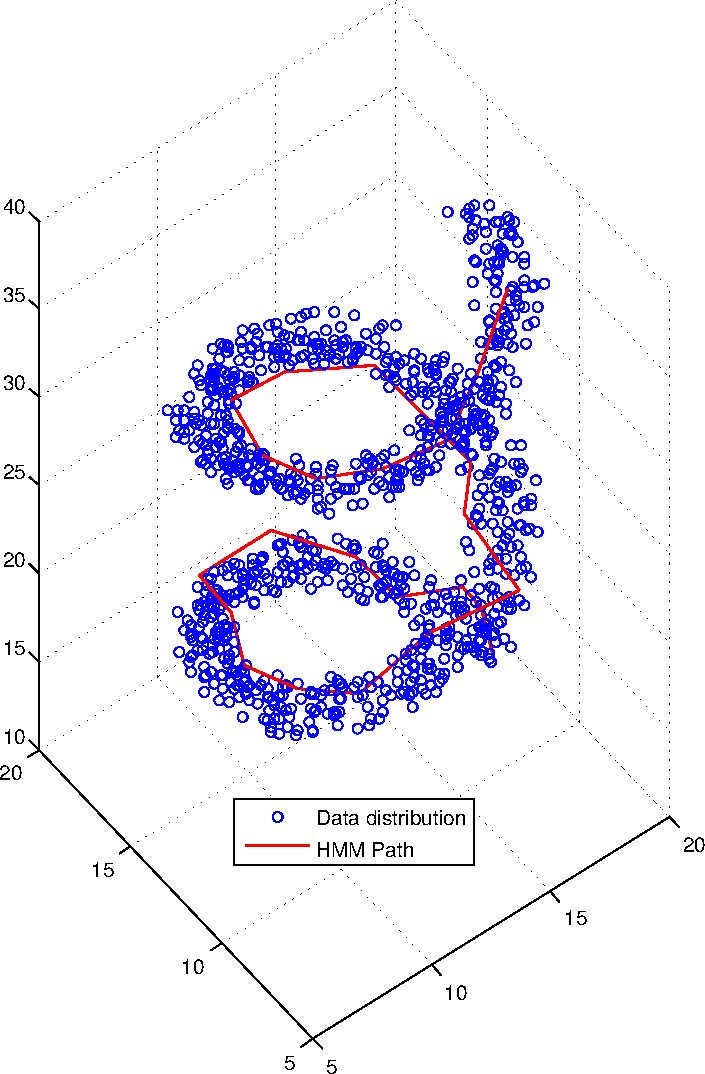
\includegraphics[width=0.3\textwidth]{Graphics/ch6/spire}
		\caption{\ac{HMM} path computed inside a density distribution defined by an helix.}
		\label{fig:spire}
	\end{center}
\end{figure}

Afterwards, we wanted to demonstrate how these paths adapt to three-di\-men\-sio\-nal structures. In this case, we created a helix-shaped point distribution in Fig.~\ref{fig:spire}. Since we need per-voxel intensity values (probailities) to estimate the paths, we have approximate this by the number of points within each voxel over the total number of points. By setting $\mathbf{p}_0$ to the point on the helix distribution with smallest $z$ coordinate, and $\mathbf{p}_N$ to the one with maximum $z$, we trace the path shown in Fig.~\ref{fig:spire}. This paths adapt to the distribution and follows it consistently until it reaches the attractor at the top of the helix.


\begin{figure}[htp]
	\centering
	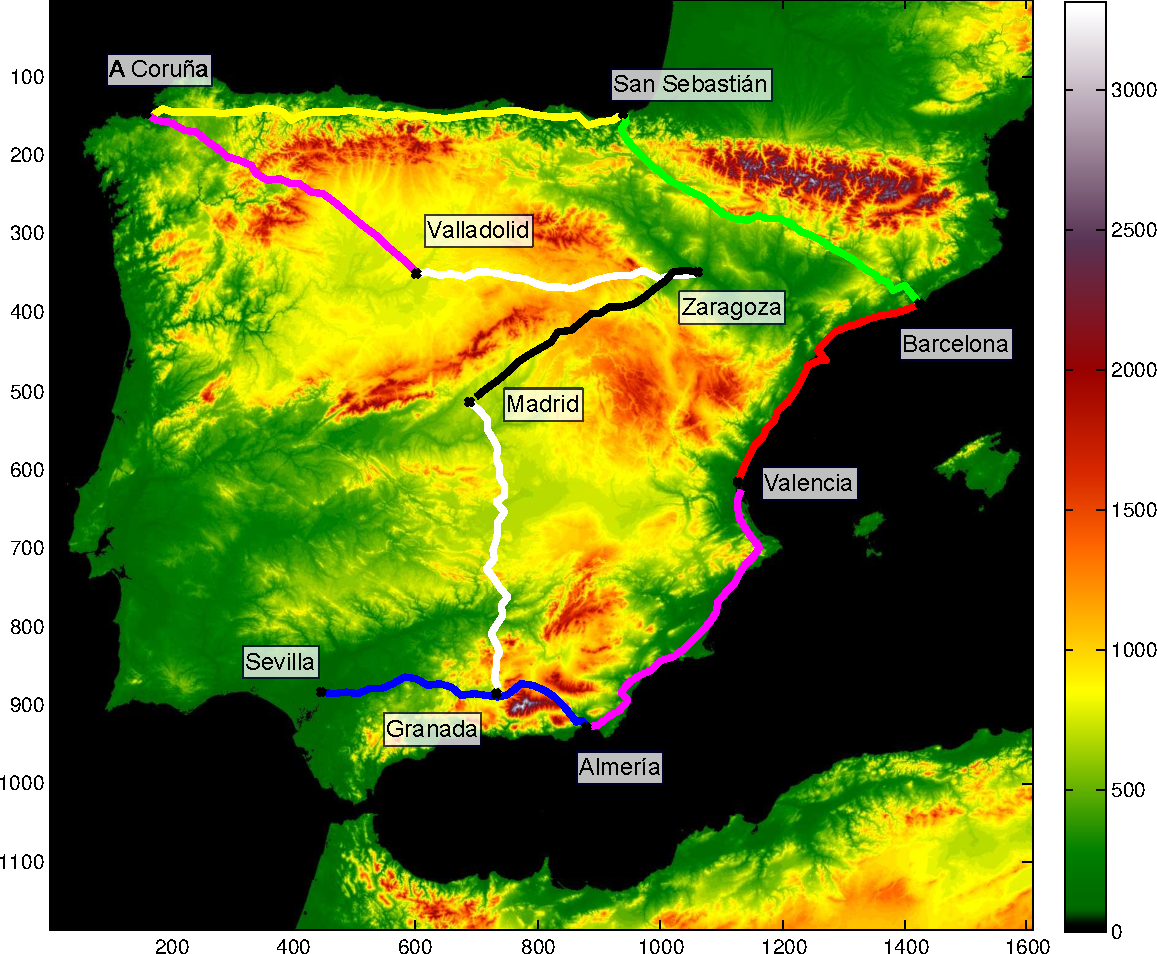
\includegraphics[width=0.7\textwidth]{Graphics/ch6/spain.pdf}
	\caption{Simulation of the \ac{HMM}-based path tracing over an Iberian Peninsula height map, interconecting different cities.}
	\label{fig:spainmap}
\end{figure}

Finally, and prior to the three-dimensional brain images, we test the algorithm on a bidimensional real-world example: a digital elevation model of the Iberian Peninsula. The image was acquired by the LANDSAT SRTM30+ mission, and its intensity represents height. We tested multiple paths by establishing sequentially $\mathbf{p}_0$ and $\mathbf{p}_N$ in ten different cities. The paths shown at Figure~\ref{fig:spainmap} optimize both the distance and height variation as well as resembling -in most cases- the roads that connect these cities in the real world. Given the dimensions of the image, in this case, the L2-norm of the support ball has been set to $r=30$. 


\subsection{Experiment 4: Feature Selection using \acs{HMM} Paths}
In Experiment 4 we begin to apply the \ac{HMM} paths to real \ac{MRI} images from the \adnimri{} dataset. We have first defined a set of paths over the DARTEL template, which we call the canonical paths. The canonical paths follow the anatomy of a normal subject to whom all other images have been registered. Therefore, the location of the different nodes on the paths are fixed throughout the general anatomy of all images, and we could characterize the differences between classes by analysing the intensity distribution on these paths --in other words, the tissue density--. In short, we apply the canonical paths as a feature selection algorithm to the different images. 

To start with, we will take all the $180\times360=64800$ canonical paths computed in all  spatial directions defined by $\varphi\in[0,360]$ and $\theta\in[-90,90]$. These paths will be used to select the voxel intensities where the nodes are placed, as in the original \ac{SBM}. Due to the influence of the different variables (trace of the paths, stop condition), the amount of values varies from 2 to several tens. First we will test the accuracy achieved by each path itself, using the set of intensities as features in a \ac{SVC} classifier. The accuracy reached by each path is represented by colour in Figure~\ref{fig:accuracyMap}. 

\begin{figure}
	\begin{center}
		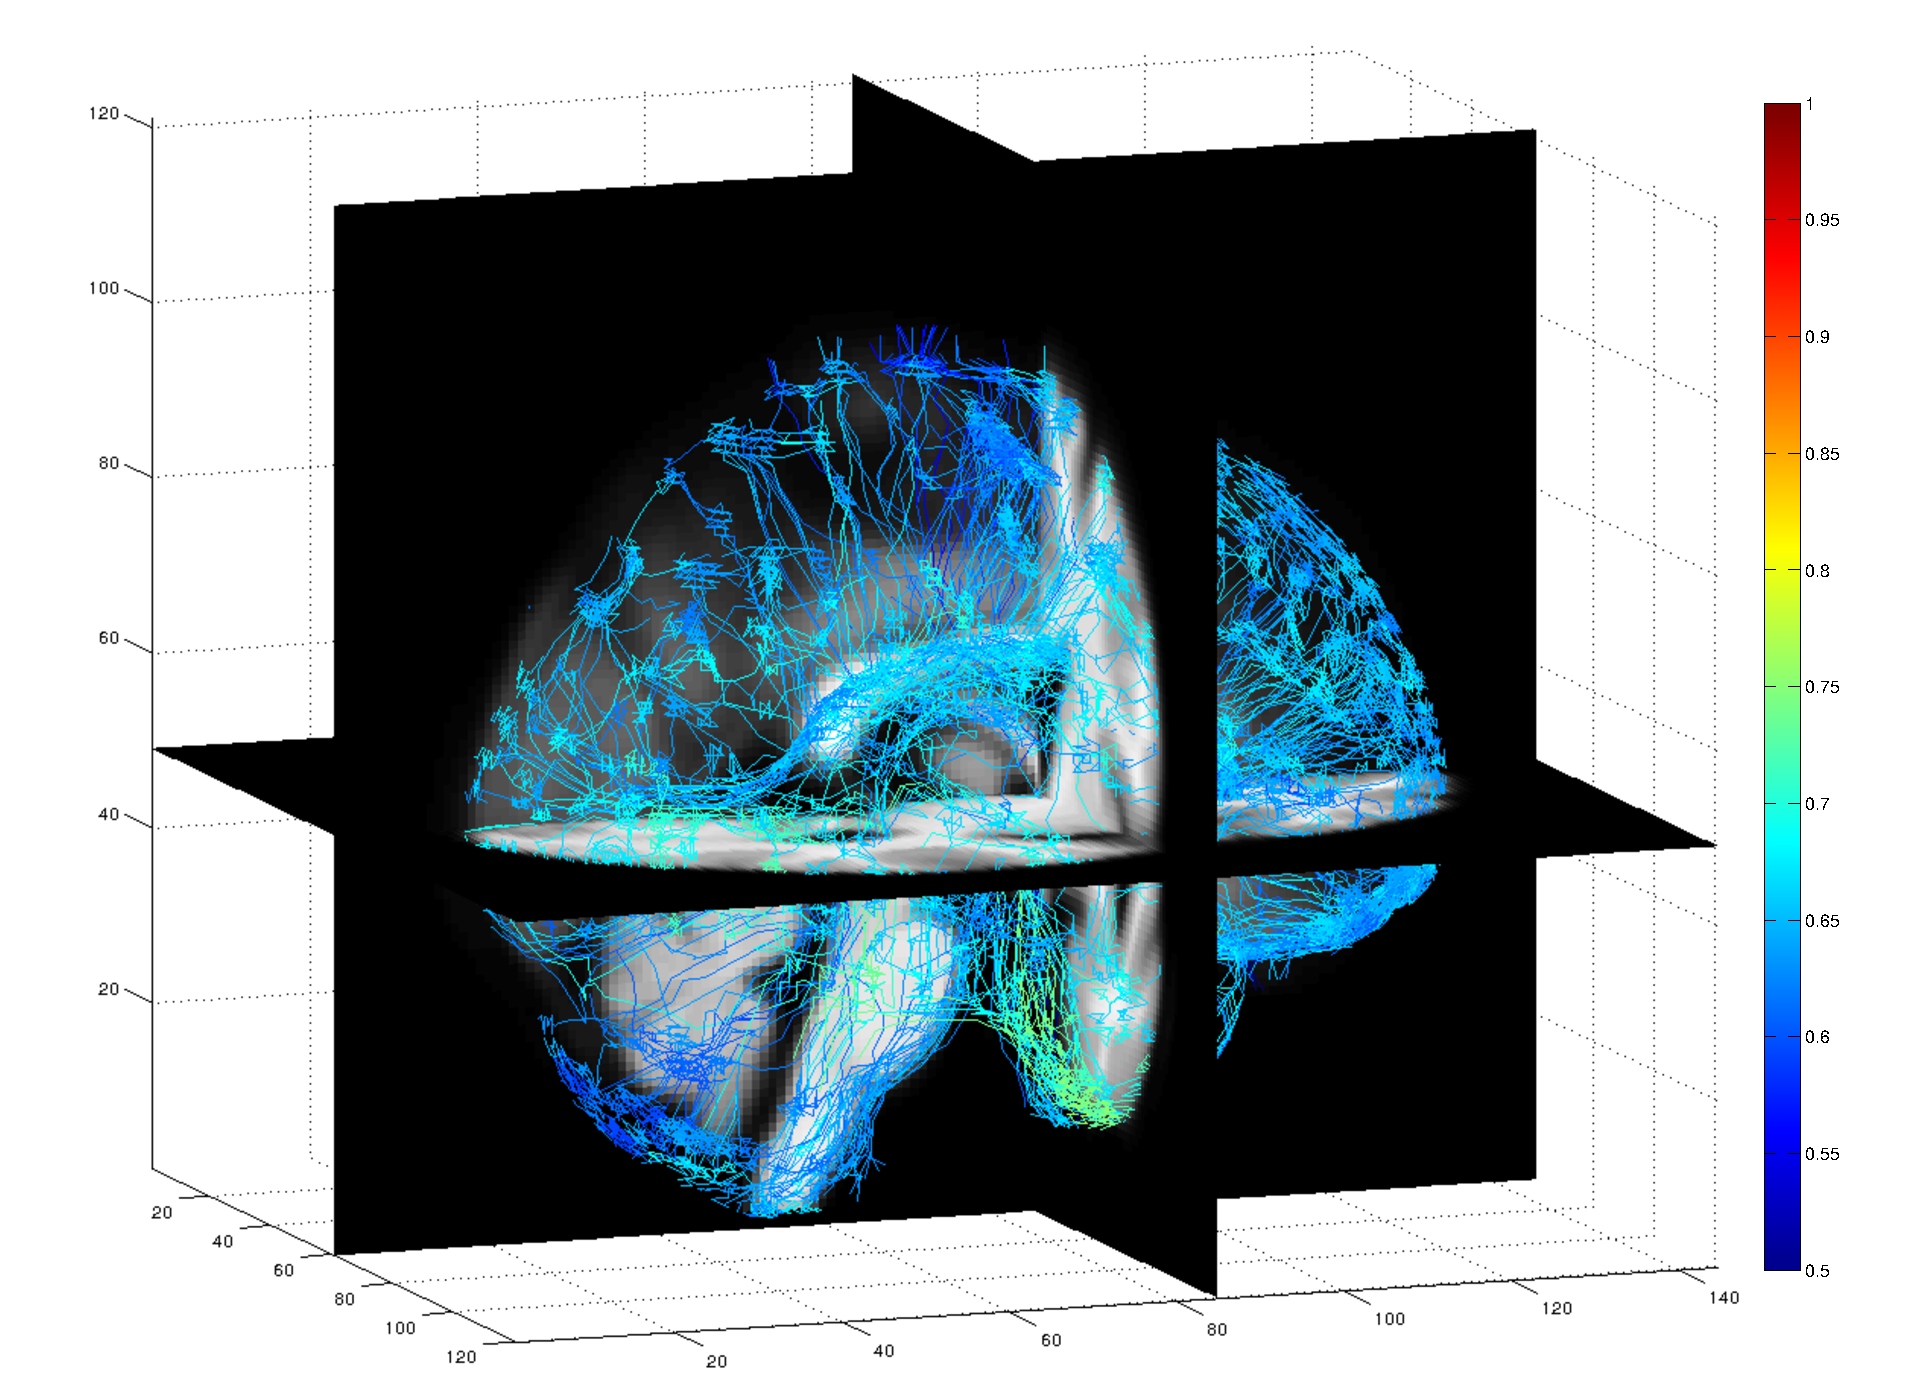
\includegraphics[width=\columnwidth]{Graphics/ch6/accuracyPaths2}
		\caption{canonical paths computed in each direction ($\theta,\varphi$). Each path's colour represent the accuracy in a differential diagnosis. Only one in every five paths are shown for clarity purposes.}
		\label{fig:accuracyMap}
	\end{center}
\end{figure}

The highest performance is achieved by some of the light green paths that cross the temporal lobe, where they reach a decent accuracy up to $0.8028\pm0.0873$. Compared to the \ac{VAF} approach obtained in the \adnimri{} dataset using T1-weighted images, under the AD vs NOR scenario ($0.789 \pm 0.066$ accuracy), this is a dramatic feature reduction while increasing the performance of the system. 

Then, we want to test whether using all the intensities contained within the highest scoring paths can increase this raw performance. To do so, we select the paths that achieved accuracies $\ge0.7$, and afterwards, we used a $t$-test over the set of intensities selected by these paths. We used a threshold $|t|>1.96$ ($p<0.05$) and all the significant intensities were used to construct a new training set. The performance for using either all voxels in the selected paths or only the significant voxels is presented at Table~\ref{tab:accHMMPaths}, for left, right and both sides. 

\begin{table}
	\myfloatalign
	\begin{tabular}{llccc}
		\toprule
		\tableheadline{Selection} & \tableheadline{Side} & \tableheadline{Accuracy} & \tableheadline{Sensitivity} & \tableheadline{Specificity} \\ \midrule
		\multirow{3}{*}{All} & Left & $0.769 \pm 0.035 $ & $0.717 \pm 0.061$ & $0.822 \pm 0.057$\\
		& Right & $0.792 \pm 0.080 $ & $0.706 \pm 0.120$ & $0.878 \pm 0.101$\\
		& Both & $0.806 \pm 0.069 $ & $0.733 \pm 0.073$ & $0.878 \pm 0.097$\\
		\midrule 
		\multirow{3}{*}{$t$-test}& Left & $0.733 \pm 0.037 $ & $0.694 \pm 0.099$ & $0.772 \pm 0.124$\\
		& Right & $0.781 \pm 0.085 $ & $0.711 \pm 0.122$ & $0.850 \pm 0.083$\\
		& Both & $0.828 \pm 0.054 $ & $0.794 \pm 0.095$ & $0.861 \pm 0.039$\\
		\bottomrule
	\end{tabular}
	\caption[Performnace values for using the \acs{HMM} paths in feature selection.]{Performance values ($\pm$SD) for the selected paths as features. First three rows correspond to using all intensities in the selected paths, and the following rows use only significant intensities (asessed by $t$-test).} 
	\label{tab:accHMMPaths}
\end{table}

Finally, we proceed as in the original \ac{SBM} article \cite{Martinez-Murcia2015}, by computing different \ac{SBM} measures using each set of intensities $V_{\theta,\varphi}$ selected by the \ac{HMM} path at the direction of the attractor $(\theta,\varphi)$. We will compute the average, entropy and kurtosis measures, as well as an additional variance term, which proved to be a good approach. An example of the computed maps is provided in Figure~\ref{fig:hmmstatmaps}.

\begin{figure}
\centering
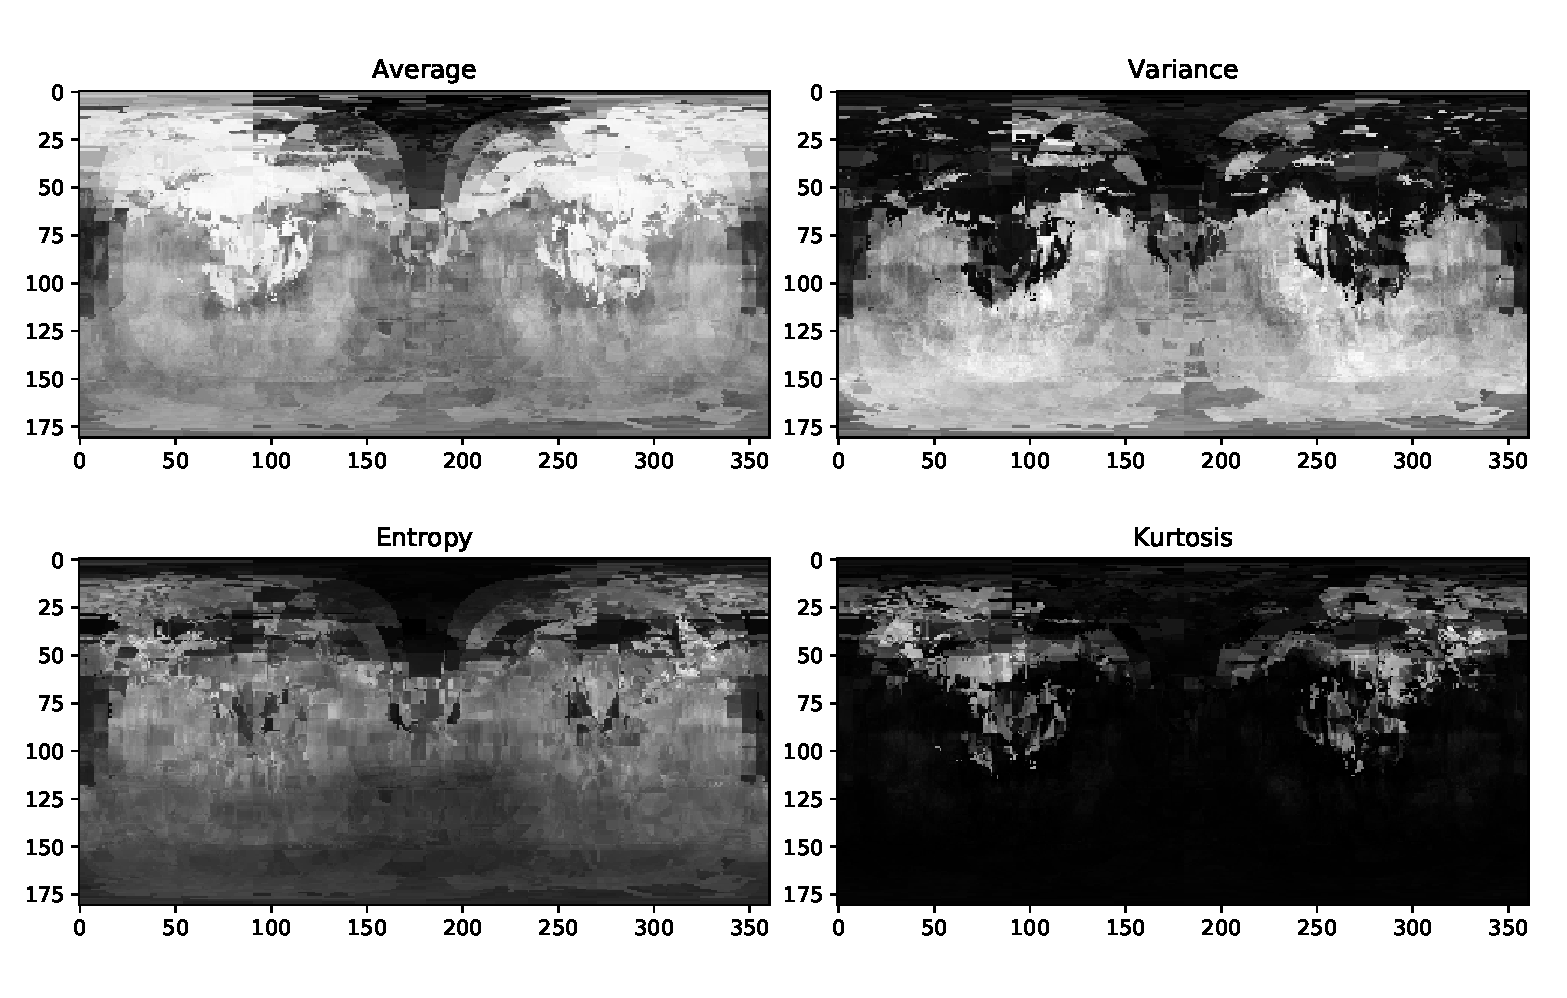
\includegraphics[width=\linewidth]{Graphics/ch6/HMMStatMaps}
\caption{Example of the resulting hybrid \acs{HMM}-\acs{SBM} texture maps.}
\label{fig:hmmstatmaps}
\end{figure}

The resulting maps are very different from the original \ac{SBM} ones, and the different structures cannot be so easily located. This is mainly due to the adaptivity of the \ac{HMM} paths, featuring a large number of twists and turns in their direction, and making them less powerful for visualization. However, the performance of using these hybrid \ac{HMM}-\ac{SBM} maps can still be high, as we can find at Table~\ref{tab:HMMsbm_perf}. 

\begin{table}
	\myfloatalign
	\begin{tabular}{lccc}
		\toprule
		\tableheadline{Feature} & \tableheadline{Accuracy} & \tableheadline{Sensitivity} & \tableheadline{Specificity} \\ \midrule
		Average & $0.594 \pm 0.062 $ & $0.661 \pm 0.121$ & $0.528 \pm 0.106$\\
		Variance & $0.750 \pm 0.064 $ & $0.633 \pm 0.131$ & $0.867 \pm 0.102$\\
		Entropy & $0.603 \pm 0.069 $ & $0.661 \pm 0.071$ & $0.544 \pm 0.125$\\
		Kurtosis & $0.756 \pm 0.105 $ & $0.733 \pm 0.165$ & $0.778 \pm 0.150$\\
		\bottomrule
	\end{tabular}
	\caption{Performance values ($\pm$SD) for the hybrid \ac{HMM}-\ac{SBM} maps, using some statistical measures.} 
	\label{tab:HMMsbm_perf}
\end{table}

\subsection{Experiment 5: Texture \acs{SBM} Maps based on \acs{HMM} Paths}
After evaluating the \ac{HMM} paths as a feature selection method, and the hybrid \ac{HMM}-\ac{SBM} maps, we want to compute new texture maps, similar to the approach used in the \ac{VRLBP} extension, but using a path-based \ac{GLCM}.  To do so, we will derive a \ac{GLCM} from each of the canonical paths, and extract one single value per texture feature and direction, which allow us to construct texture \ac{SBM} maps. In Table~\ref{tab:texture} we show the performance values for the maps built using each of the texture features proposed in Section~\ref{sec:rtextfeat}

\begin{table*}
	\myfloatalign
	\begin{tabularx}{\textwidth}{Xccc}
		\toprule
		\tableheadline{Feature} & \tableheadline{Accuracy} & \tableheadline{Sensitivity} & \tableheadline{Specificity} \\ \midrule
		Energy & $0.689 \pm 0.061 $ & $0.700 \pm 0.115$ & $0.678 \pm 0.073$\\
		Entropy & $0.675 \pm 0.101 $ & $0.672 \pm 0.115$ & $0.678 \pm 0.159$\\
		Correlation & $0.672 \pm 0.068 $ & $0.672 \pm 0.112$ & $0.672 \pm 0.100$\\
		Contrast & $0.733 \pm 0.060 $ & $0.689 \pm 0.126$ & $0.778 \pm 0.105$\\
		Homogeneity & $0.697 \pm 0.058 $ & $0.700 \pm 0.115$ & $0.694 \pm 0.106$\\
		Dissimilarity & $0.711 \pm 0.085 $ & $0.678 \pm 0.110$ & $0.744 \pm 0.102$\\
		Difference Variance & $0.736 \pm 0.070 $ & $0.683 \pm 0.098$ & $0.789 \pm 0.090$\\
		Difference Entropy & $0.725 \pm 0.122 $ & $0.683 \pm 0.176$ & $0.767 \pm 0.114$\\
		IDN & $0.719 \pm 0.065 $ & $0.683 \pm 0.108$ & $0.756 \pm 0.105$\\
		IDMN & $0.717 \pm 0.076 $ & $0.678 \pm 0.125$ & $0.756 \pm 0.084$\\
		\bottomrule
	\end{tabularx}
	\caption{Performance values ($\pm$SD) for each of the 10 texture features.} \label{tab:texture}
\end{table*}

Difference variance achieves here the higher accuracy, $0.736 \pm 0.070$, a value similar to the \ac{VAF} approach in this database. The performance achieved by these texture features is always higher than $65\%$ (most of them above $70\%$) which reveals a discrete discrimination ability, although much smaller than the one shown by the \ac{HMM} paths, used as feature selection tool. 

\section{Discussion}
\subsection{Spherical Brain Mapping}
The Spherical Brain Mapping defines a completely new approach to visualization and feature extraction of segmented \ac{MRI} images. We have tested the original maps (including the \ac{VRLBP} approach) in Experiment 1, and its layered extension in Experiment 2. 

From the analyses performed, we can conclude that the most significant changes occur mainly in the \ac{GM} tissue (see fig.~\ref{fig:performance}), although some maps perform better with \ac{WM}. According to the widely documented structural changes due to Alzheimer's Disease, these occur mainly in \ac{GM} \cite{Misra2009,Baron2001,Pievani2013,Stoeckel04,han2006reliability,Fischl2004}, which is consistent to what we found, and the significance found in \ac{WM} might be the ``negative'' influence of the \ac{GM} loss. That is revealed in the statistical significance analysis of Figures~\ref{fig:tmaps} and \ref{fig:tmapvrlbp}, where the $t$-values in \ac{WM} are negative in the areas where we found positive values in \ac{GM} maps. This can be also appreciated in the layered approach, at Figure~\ref{fig:tmaplayered}. 

\begin{figure}[htp]
	\centering
	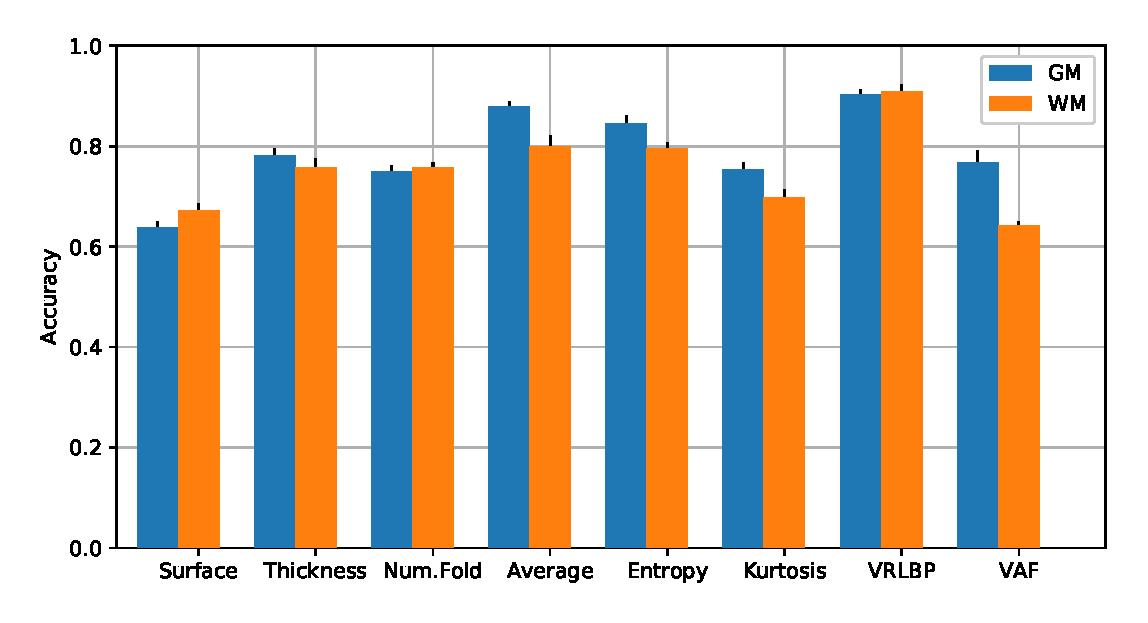
\includegraphics[width=0.8\columnwidth]{Graphics/ch6/12-performance}
	\caption{Performance at the operation point for the different mappings over the \acs{GM} and \acs{WM}, compared with the performance of \acs{VAF}.}
	\label{fig:performance}
\end{figure}

The mappings defined at Sections~\ref{sec:mapping}, \ref{sec:layered} and \ref{sec:vrlbp} model a series of properties of the tissues crossed by the mapping vector $\mathbf{v}_{\theta,\varphi}$. We classified all the \ac{SBM} measures in three groups: morphological (surface, number of folds and thickness), statistical (average, variance, entropy or kurtosis) and texture (\ac{VRLBP}). The morphological approaches are easily interpreted, since they represent things such as the surface of the tissue, the complexity of the tyri and sulci folding, and the thickness. Surface and thickness are defined in a similar way to other widely-used software, such as Freesurfer~\cite{Dale1999,Fischl2004}, although are less powerful in defining this complexity, due to the limitations in our rectilinear mapping. 

Therefore, the surface measure is not a faithful representation of the surface of the cortex, as it can be seen in Fig.~\ref{fig:masksGM}, and later in the $t$-maps at Fig.~\ref{fig:tmaps}. That is why its performance is so small due to the superposing gyri and sulci, and better for \ac{WM}, where it achieves a higher level of detail. As for the thickness measure, it cannot achieve the same level of detail of the Freesurfer's measures, although gathering much more information than other morphological approaches. Nevertheless, the thickness of these tissues can still be very descriptive, and it achieves a decent performance in the classification analysis. The number of folds is the last of these morphological measures. It is intended to measure the complexity of the cerebral cortex, although judging by its performance, it does not do a very good job. 

The statistical measures, especially average, achieve higher performance in the classification analysis. That might be due to the precision of the numbers used. Whereas in the morphological features we obtained integers (as they count the number of voxels or zero-crossings), in the statistical measures values such as average or entropy compute high-precision floating values. This can help in further computation, although values such as kurtosis are outperformed by, for example, thickness. 

The average is the best-performing measure in this group, and can be interpreted as the average amount of tissue -even tissue density- in the direction $(\theta,\varphi)$. A comparison between the densities of the tissues in \ac{AD} and \ac{CTL} can reveal the neurodegeneration and tissue loss typically associated with the disease. This is perhaps why in the significance analysis we found high absolute $t$-values in areas typically affected by \ac{AD}, such as the mid temporal lobe, amygdala, hippocampus, parahippocampal gyrus or some structures of the basal ganglia, such as caudate nucleus, globus pallidus or putamen \cite{Dubois2007,Pievani2013}. 

Entropy is a more complex statistical concept that comes from information theory, but is usually related to the amount of information, or in other words, the ``randomness'' of a source. In our particular case it could be interpreted as a measure of texture, that is, the grey-level variability in the direction of $\mathbf{v}_{\theta,\varphi}$. These maps perform very similar to the average ones in both \ac{GM} and \ac{WM}, suggesting that the entropy  accounts here for the tissue density as well. 

The last measure of this group, the kurtosis, is also the less performing statistical feature. It is a fourth-order statistic that might be interpreted as the ``peakedness'' of a probability distribution. In the case of the \ac{SBM} maps, it models how abrupt the intensity changes in the direction $\mathbf{v}_{\theta,\varphi}$ are. This relates kurtosis to the number of folds, and as in this case, the performance is also small. This is probably due to the fact that the main neurodegenerative processes are better modelled by atrophy-related measures, such as average or thickness, than with the complexity measures such as number of folds, kurtosis. 

Finally, the \ac{VRLBP} gathers not only the intensity values in the mapping vector, but also its neighbourhood, thanks to the helical sampling applied. This is probably why the \ac{VRLBP} achieve the best performance in the classification analysis, with accuracies above $0.9$ for both \ac{GM} and \ac{WM} tissues. Texture can also be associated with changes in the tissue density or distribution, which could lead to this higher performance. The most relevant regions in the \ac{VRLBP} correspond to small areas in the temporal lobe, amygdala and hippocampus, where the neurodegeneration could be causing the texture changes that we detected. 

The breakdown of the \ac{SBM} maps into several layers might be considered a enhancement over the single maps, thanks to the level of detail achieved at different depths. However, it barely outperforms ($0.874 \pm 0.021$ accuracy) the single-layer \ac{SBM} average measure, much less the best-performing \ac{VRLBP}. Therefore, its only contribution is a better visualization of overlapping structures. The most discriminant layer in a four-layer decomposition is layer 2, which is consistent with the presence of some \ac{AD}-related organs such as the hippocampus, amygdala or putamen. 

% DONE

%%%%%%%%%%%%%%%%%%%%%%%% 
%
%\begin{figure*}[htp]% ROC
%	\centering
%	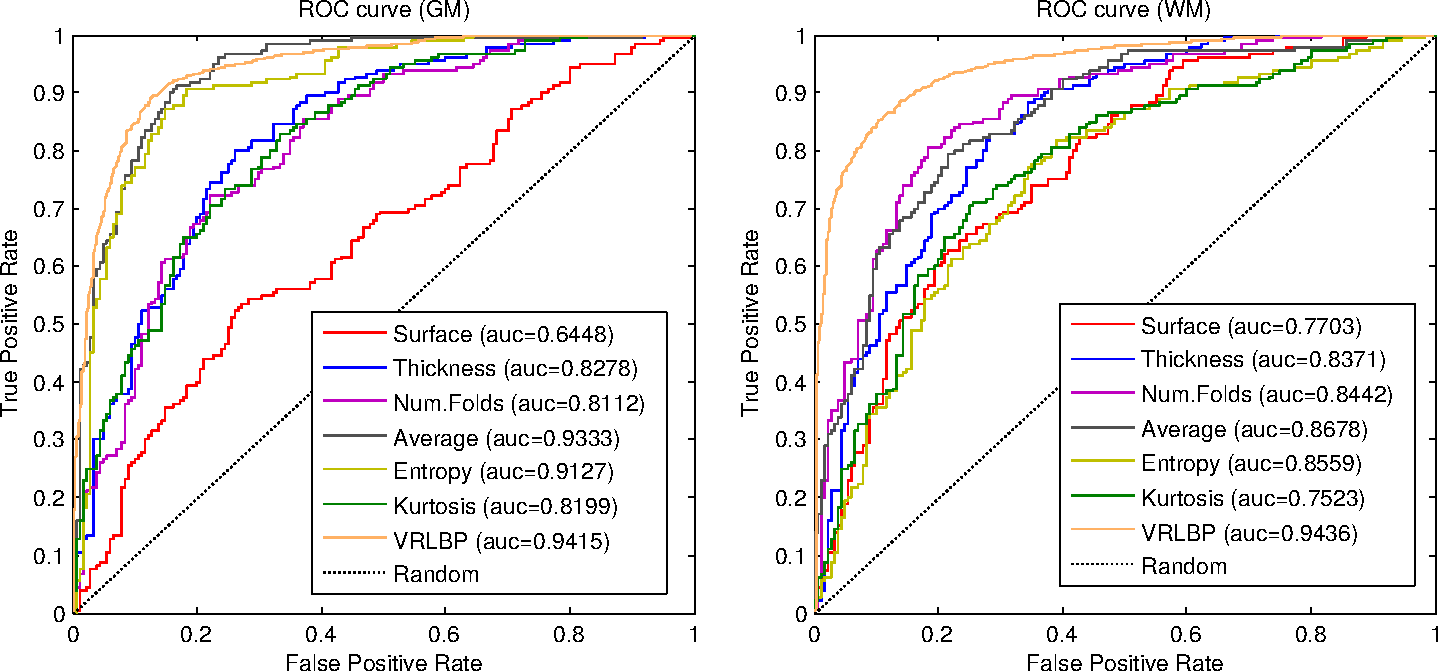
\includegraphics[width=0.8\textwidth]{Graphics/ch6/13-ROC}
%	
%	\caption{ROC curves of the different mappings for the \ac{GM} and \ac{WM} tissues.}
%	\label{fig:roc}
%\end{figure*}
% BORRO ROC PORQUE NO SE DEFINEN NI USAN EN NINGÚN OTRO SITIO. 
%Finally, in order to have another look at the performance of our mappings, the ROC curves of each type are presented in Figure~\ref{fig:roc}. There we can see how the VRLBP approach outperforms all the other measures, specially in the case of \ac{WM} tissue. In \ac{GM}, Average and Entropy present values really close to VRLBP, as expected. Conversely, the poorest performance is achieved by the Kurtosis and Surface mappings, however the Surface performs better in \ac{WM} than in \ac{GM}. These results confirm the performance values presented in  Table~\ref{tab:perfProj} and Figure~\ref{fig:figureGM}, making our proposed mapping framework a reasonable choice for obtaining both a visual interpretation of otherwise hidden features and a significant dimensionality reduction. 


\subsection{Paths via \acs{HMM}}\label{sec:discussion}
Now we will discuss the \ac{HMM} paths proposed in Section~\ref{sec:hmmpaths}, whose results were analysed in Experiments 3, 4 and 5. The paths were proposed as a curvilinear substituent of the \ac{SBM} mapping vector $\mathbf{v}_{\theta,\varphi}$, capable of adapting to the structure changes found in the brain. Our paths $\mathbb{P}_{\theta,\varphi}$ are built upon a minimun intensity variation pathway that starts at the \ac{AC}, and follows the orientation of an attractor placed in the limits of the image at the spherical coordinate pair $(\theta,\varphi)$. 

There is a fundamental reason why \ac{AC} is the best choice as first node of the paths: it is a privileged position where the left and right hemispheres are connected. A different point would lead to suboptimal paths, whose construction might be quickly interrupted by the abrupt changes at the ventricles, and therefore, the resulting set of paths would not cover the entire brain. 

It is important to note that these are not functional connectivity maps like \acf{DTI} fibre tracts, which have also been used in the diagnosis of \ac{AD} \cite{Grana2011,Medina2008}. \ac{DTI} tracts are based upon difussion images that quantify the water molecule motion --in magnitude and direction-- throughout a tensor processing. Our \ac{HMM} path definition, on the other hand, only characterize grey level connectivity in \ac{MRI} images, starting in white matter and progressively transitioning to \ac{GM}, oriented in a fixed direction. This means that, although images like Figure~\ref{fig:accuracyMap} could resemble \ac{DTI} fibres, they are not related at all, and their utility as a feature selection tool is completely different. 

Our paths demonstrated in Experiment 3 that they can adapt easily to two and three-dimensional images, and even to the statistical distribution of points in space (as in the helix example). They were successfully tested against a real world example, aimed at tracing roads on a height map of the iberian peninsula, with the result of paths that closely resemble real roads in which the minimum variation in height is key. 

\begin{figure}
	\begin{center}
		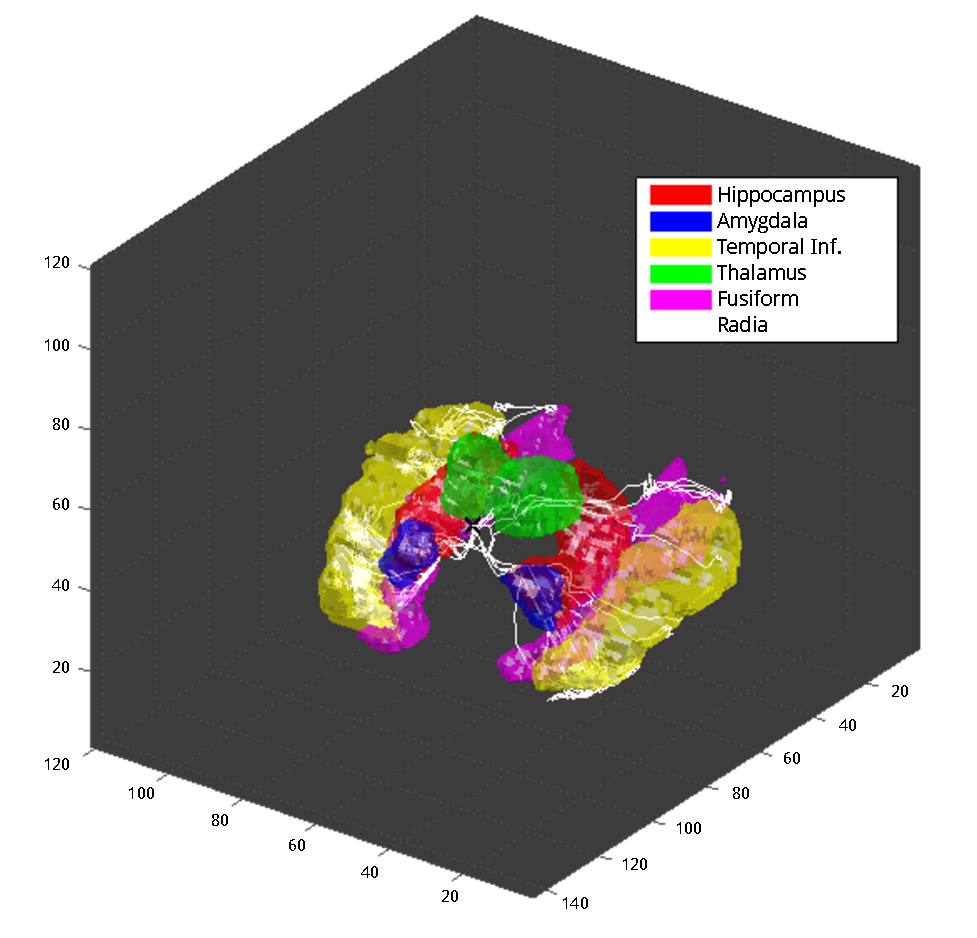
\includegraphics[width=0.9\textwidth]{Graphics/ch6/radia&structures}
		\caption{Paths that obtain more than 75\% accuracy, and a three-dimensional representation of the structures crossed by them.}
		\label{fig:bestPaths}
	\end{center}
\end{figure}

Later, in Experiment 4, we used the \ac{HMM} paths as a feature selection tool to construct the set of selected intensities $V_{\theta,\varphi}$, as in the original \ac{SBM}. Individual paths as well as a the pooled intensities of all paths in a hemisphere were tested using a \ac{SVC}. The differences between intensity sets in \ac{AD} and \ac{CTL} were significant enough to achieve accuracies over 80\% in some paths. The paths that achieved more than 75\% accuracy are shown in Figure~\ref{fig:bestPaths}, along with the rendered structures crossed by them, according to the \ac{AAL} brain atlas \cite{Tzourio-Mazoyer2002}. 

The structures that are crossed by the best-performing paths are the Hippocampus, Amygdala, Thalamus, Fusiform and Inferior Temporal Gyrus. \ac{GM} loss in the hippocampus has been extensively reported in the literature \cite{Dubois2007,Baron2001,Jong2008}, as well as its surrounding structures (Amygdala, parahippocampal gyrus and Fusiform) \cite{Baron2001}. Some studies have also reported neurodegeneration at the Thalamus and Putamen, also related to early \ac{AD} \cite{Jong2008}, and in advanced \ac{AD}, atrophy in most of the neocortex \cite{Dubois2007,Baron2001,Jong2008}. However, pooling all the intensities selected by these paths together did not increase the performance achieved by the best performing paths. 

The last test of Experiment 4 was the hybrid \ac{SBM}-\ac{HMM} maps. Average, entropy, kurtosis and variance maps were tested, and we found that they were discriminant (accuracy above 70\% in most cases), yet not very powerful. This is however coherent with the definition of the paths, where the intensity changes are small and progressive, and therefore, higher order statistics that focus on this (such as variance or kurtosis) are more representative of this behaviour. 

Finally, we tested the \ac{HMM} paths' application to compute radial \ac{GLCM} and texture features at Experiment 5. Here we saw that the performance achieved with any of the texture feature maps was smaller than using the best paths themselves, or even the most significant paths. However, the real utility of the texture \ac{HMM} maps could reside in its application to longitudinal studies. Texture has been already related to the evolution of \ac{AD} \cite{sikio2015mr}, and so, the evolution of the generated texture maps over the canonical paths throughout time could be a good indicator of the progression of \ac{AD}. 

Further improvements could be made by computing an independent set of paths per subject, and then extract morphological measures such as curvature or torsion, or extend the computation of textural features to longitudinal studies, as we mentioned previously. This seem a very promising approach that will be tested in future works. 

\subsection{\acs{SBM} Framework Comparison}
To obtain a general view of the \ac{SBM} and its extension within the state of the art, in Table~\ref{tab:comparison2} we present some of the best results that have been already commented. We first present the values for the \ac{VAF} approach \cite{Stoeckel04} in T1, \ac{GM} and \ac{WM} images. Then, we present the performance of the average and \ac{VRLBP} maps of our \ac{SBM}, and the \ac{HMM} paths, both as feature selection tool (individual paths and selected features from the paths), the hybrid \ac{HMM}-\ac{SBM} tool (variance and kurtosis) and the best scoring texture feature (difference variance). 

Afterwards, we provide reference values of some state of the art methodology that has been tested against the \adnimri{} database. These are: LVQ) a Learning Vector Quantization (LVQ) \cite{Ortiz2013} used to model the tissue distribution of \ac{CTL} and \ac{AD} images and project the images to a new space, just to use the projections in a \ac{SVC}; and SCA) the Spatial Component Analysis proposed in \cite{Illan2014}, a bayesian network modelling of the dependencies between affected regions (or spatial components) in \ac{AD}. 

\begin{table}
	\myfloatalign
	\begin{tabular}{lllccc}
		\toprule
			\tableheadline{App.} & \tableheadline{Feature} & \tableheadline{Tis.} & \tableheadline{Accuracy} & \tableheadline{Sensitivity} & \tableheadline{Specificity} \\ \midrule
			\multirow{3}{*}{\ac{VAF}}  & \multirow{3}{*}{Intensity} & T1 & $0.789 \pm 0.066 $ & $0.767 \pm 0.094$ & $0.811 \pm 0.099$\\
			 & & \ac{GM} &  $0.768 \pm 0.011$ & $0.752 \pm 0.016$ & $0.785 \pm 0.016$ \\
			 & & \ac{WM} & $0.642 \pm 0.009$ & $0.668 \pm 0.012$ & $0.617 \pm 0.013$ \\
			\midrule
			\multirow{4}{*}{\ac{SBM}} & \multirow{2}{*}{average} & \ac{GM}  & $0.879 \pm 0.005$ & $0.897 \pm 0.006$ & $0.861 \pm 0.006$ \\
			& &\ac{WM}  & $0.800 \pm 0.011$ & $0.802 \pm 0.013$ & $0.798 \pm 0.009$ \\ 
			\cline{2-6}
			&  \multirow{2}{*}{\ac{VRLBP}}&\ac{GM}  & $0.903 \pm 0.010$ & $0.890 \pm 0.012$ & $0.916 \pm 0.018$ \\
			& &\ac{WM} & $0.909 \pm 0.014$ & $0.899 \pm 0.028$ & $0.919 \pm 0.018$ \\ \midrule
			\multirow{5}{*}{\ac{HMM}} & Ind. Paths & T1 & $0.806 \pm 0.069 $ & $0.733 \pm 0.073$ & $0.878 \pm 0.097$\\
			& Sel. Paths & T1 & $0.828 \pm 0.054 $ & $0.794 \pm 0.095$ & $0.861 \pm 0.039$\\
			& Variance & T1 & $0.750 \pm 0.064 $ & $0.633 \pm 0.131$ & $0.867 \pm 0.102$\\
			& Kurtosis & T1 & $0.756 \pm 0.105 $ & $0.733 \pm 0.165$ & $0.778 \pm 0.150$\\
			& D. Variance & T1 & $0.736 \pm 0.070 $ & $0.683 \pm 0.098$ & $0.789 \pm 0.090$\\
			\midrule 
			\multirow{3}{*}{Other} & LVQ & \ac{GM} & $0.869 \pm 0.101$ & $0.822\pm0.120$ & $0.890\pm0.102$ \\ 
			\cline{2-6}	
			 &\multirow{2}{*}{SCA} & \ac{GM} & $0.880 \pm0.0^* $ & $0.926\pm0.0^* $ & $0.845\pm0.0^*$ \\ 
			 & & \ac{WM} &$0.808 \pm 0.0^*$ & $0.817\pm0.0^*$ & $0.800\pm0.0^*$ \\ 	
			\bottomrule
		\end{tabular}
	\\
	{\small $^*$ SCA used leave-one-out cross-validation. SD is 0.}
		\caption{Comparison between our algorithm performance values (best values for selected voxels in all paths and texture features) ($\pm$SD) and other methods in the bibliography} \label{tab:comparison2}
	\end{table}

The original \ac{SBM} achieve generally better results than its counterpart using \ac{HMM} paths. That gives us an idea that the utility of these paths is not to generate the \ac{SBM} maps, but to characterize the structure itself of the brain, which could have applications when applying a morphological characterization of the individual set of paths computed over each subject, or even in segmentation of the images. The seven \ac{SBM} measures proposed here have been of great utility, clearly outperforming the \ac{VAF} approach, and achieving results similar to state-of-the-art methodology in the field, while providing a useful two-dimensional representation of the brain. This is especially the case of the \ac{VRLBP}, which according to the statistical significance analysis, was able to locate major differences in very small regions of the brain. 

To end with, we want to remark that the \ac{SBM} defines a whole framework that can easily be extended with different strategies. We already proposed the layered extension or the neighbourhood helical sampling that we tested with the \ac{VRLBP}, but many others can be made. Higher order statistics on the set of intensities $V_{\varphi,\theta}$, or the computation of \acp{GLCM} around the mapping vector can focus on different properties of the structure of the image. We could even, instead of using the \ac{HMM} paths, use the fibre tracts defined in \ac{DTI} modalities to compute features that are related to brain connectivity, and could be potential indicators of neurodegeneration, or even apply \ac{SBM} to other imaging modalities such as \ac{PET} or \ac{SPECT}, where the structural information is not always present.
% DONE
	